\documentclass[a4paper]{jpconf}
\usepackage{amsmath}
\usepackage{amssymb}
\usepackage[UKenglish]{babel}
\usepackage{graphicx}
\usepackage{hyperref}
\hypersetup{colorlinks=false, bookmarks=true}
\usepackage{float}
\usepackage{comment}
\usepackage{caption}
\usepackage[skip=0.5ex]{subcaption}
\usepackage{xcolor}

\hyphenation{few-femto-second}

\begin{document}
%\maketitle

\twocolumn[

\pagenumbering{arabic}
\title{Modelling of nonlinear light up-conversion from intense femtosecond laser pulses}
\author{David Amorim (University of Glasgow)}
\address{DESY Summer Student Programme 2023 \\ Group:  Attosecond Science (CFEL-ATTO) \\ Institute: Centre for Free-Electron Laser Science (CFEL)\\ Supervisor: Josina Hahne}

\begin{abstract}
Few-cycle ultraviolet (UV) laser pulses can be produced via nonlinear optical processes in noble gasses using few-femtosecond near-infrared input pulses. The theoretical modelling of these effects is challenging, however, as many common pulse propagation equations are based on approximations that do not hold for ultrashort pulses. 
This report presents numerical simulations of UV generation in the femtosecond regime using the propagation solver \textit{Luna.jl}. \par 
Despite employing a simplified gas distribution model, the simulations could reproduce general trends and qualitative features of experimentally obtained UV spectra and pulse energies. It was further demonstrated that the simulations give insights into effects that are difficult to access experimentally, such as pulse compression due to ionisation-induced self-defocusing. Additionally, the simulations were shown to be valuable in computationally investigating the effects of changing different experimental parameters, like the chirp of the input pulse, as well as design features, such as the gas confinement and pumping system. \par 
With further modifications and extensions, particularly of the gas density model, the simulations presented here could form the basis of a robust theoretical framework to complement experimental results and aid experimental design.  
\end{abstract}
]


\thispagestyle{plain}
\pagestyle{plain}
\setlength{\footskip}{20pt}

\section{Introduction}
The electronic motion associated with chemical reactions and atomic energy transitions takes place on femotsecond ($1 \text{fs} = 10^{-15} \text{s}$) to attosecond ($1 \text{as} = 10^{-18} \text{s}$) time scales. Time-resolved imaging of molecular dynamics therefore requires ultrashort laser pulses in the few-femtosecond and attosecond regime. An important type of electronic motion is that excited by the absorption of ultraviolet (UV) radiation: a variety of biochemical processes, such as DNA damage, are known to be caused by UV excitation. Generating few-femtosecond UV pulses for time-resolved measurements of UV-excited molecules plays a crucial part in further understanding and eventually controlling these effects. \par 
The CFEL-ATTO group at DESY produces ultrashort UV pulses in the femtosecond regime via third-harmonic generation (THG) in a gas cell \cite{galli2019}. This process is sensitive to a large range of parameters which affect the duration and energy of the generated UV pulses. Numerical simulations of the interactions between the laser beam and the gas can therefore be advantageous to better understand how THG takes place and how it is affected by the experimental conditions. The theoretical description of UV generation in the femtosecond regime is challenging, however, since the simplifying assumptions commonly used in pulse propagation calculations do not apply to ultrashort laser pulses. \par 
This report summarises the work carried out as part of a DESY Summer Student project focussed on producing simulations of the THG process for few-femtosecond pulses. The simulations were carried out using the propagation solver \textit{Luna.jl} (\cite{brahms2023}). The aim of the simulations was to reproduce the experimental conditions in the gas, in order to study which effects dominate the THG process and the shaping of the UV pulse. 

\section{Background}
This section gives a brief overview of key properties of ultrashort laser pulses,  THG and other relevant nonlinear optical effects, as well as the differential equation describing the propagation of ultrafast laser pulses. An in-depth treatment of these topics can be found in textbooks like \cite{keller2021, new2011}. \par 
Further, the experimental conditions for UV generations are presented, which the simulations aim to replicate. More details on the experimental work in few-femtosecond UV production carried out by the CFEL-ATTO group can be found in publications such as \cite{galli2019}. 

\subsection{Ultrashort Laser Pulses}
An ultrashort laser pulse can be described as a carrier wave at carrier frequency $\omega_0$ with an amplitude modulated by an envelope function. In the femtosecond domain the envelope may only contain a few cycles of the carrier wave. Using the analytic representation of the electric field vector, the time-domain representation of an ultrashort laser pulse can be written as 
\begin{equation}
\mathbf{E}(t, \mathbf{r}) = \mathbf{A}(t, \mathbf{r}) e^{i[ \omega_o t + \phi(t)]},
\end{equation}
where $\mathbf{A}(t, \mathbf{r})$ represents the envelope function and $\phi(t)$ is the temporal phase. The vectorial nature of the envelope takes into account the polarisation of the pulse. Similarly, the frequency-domain representation is 
\begin{equation}
\mathbf{E}(\omega, \mathbf{r}) = \mathbf{A}'(\omega, \mathbf{r}) e^{i \varphi(\omega)},
\end{equation}
where $\varphi(\omega)$ is the spectral phase. Note that the effect of the carrier term in the frequency domain is merely a shift along the frequency axis and can thus be absorbed in the definition of $\omega$. \par 
The spectral and temporal phase are commonly expanded as Taylor-series, with the symbols $\phi_n \equiv \frac{\partial^n \phi}{\partial t^n}$ and $\varphi_n \equiv \frac{\partial^n \varphi}{\partial \omega^n}$ used to denote the series coefficients. The zeroth-order terms of both expansions are the same, $\phi_0 = \varphi_0$, and correspond to the carrier-envelope phase (CEP), also known as the absolute phase. The CEP describes the phase difference between the maximum of the electric field and the peak of the envelope and is particularly relevant for few-cycle pulses. A laser pulse with no terms in $\varphi(\omega)$ higher than $\varphi_1$ is said to be transform-limited. A pulse is said to be chirped if there are nonlinear terms in $\phi(t)$ or $\varphi(\omega)$. \par 
The presence of chirp may result in both spectral and temporal broadening of the pulse envelope. A convenient measure of chirp is therefore the so-called time-bandwidth product $\Delta \omega \Delta t$, where $\Delta \omega$ is the full-width half-maximum (FWHM) of $\mathbf{A}'(\omega, \mathbf{r})$ and $\Delta t$ the FWHM of $\mathbf{A}(t, \mathbf{r})$. It can be shown that the time-bandwidth product is minimised for transform-limited, i.e. unchirped, pulses. \par 
The effects on a laser pulse when propagating through a medium are described via additional terms in the spectral phase: $\varphi(\omega) \to \varphi(\omega) + [\beta(\omega) + i \alpha(\omega)]L$, where $L$ corresponds to the propagation distance, $\beta(\omega)$ is the propagation coefficient, and $\alpha(\omega)$ is the absorption coefficient. The latter term represents an attenuation of the pulse while the former has the effect of introducing chirp (provided the Taylor-expansion of $\beta(\omega)$ has non-zero terms higher than $\beta_1$). Note that depending on the signs of the quantities involved, the chirp due to $\beta(\omega)$ will either increase or compensate the existing chirp on the pulse. Thus, an initially positively chirped pulse will further broaden upon propagation through a normally dispersive medium while a negatively chirped pulse will be compressed. The opposite effect is observed in anomalously dispersive media. The coefficient $\beta_2$ in the Taylor-expansion of $\beta(\omega)$ is of particular practical importance and generally known as group velcity delay (GVD).

\subsection{Nonlinear Optics and THG}
For most materials, the polarisation response to an electric field of moderate intensity is linear. The peak intensities reached in ultrashort laser pulses are large enough, however, for this approximation to become invalid and nonlinear polarisation components to appear. The resulting polarisation can then be represented as a combination of a linear and a nonlinear term: $\mathbf{P}(t, \mathbf{r}) = \mathbf{P}^\text{L}(t, \mathbf{r}) + \mathbf{P}^\text{NL}(t, \mathbf{r})$. \par 
The linear polarisation is given by the familiar expression $\mathbf{P}^\text{L}(t, \mathbf{r}) = \epsilon_0 \chi_e \mathbf{E}(t, \mathbf{r})$, where $\chi_e$ is the (linear) electric susceptibility. The nonlinear term, $\mathbf{P}^\text{NL}(t, \mathbf{r})$, on the other hand, is less trivial. It can be approximated using a perturbative approach in combination with a term that takes into account the effects of photoionisation, which is non-perturbative:
\begin{equation}\label{eq:p_nl}
\mathbf{P}^\text{NL}(t, \mathbf{r}) = \epsilon_0 \sum_{n=2} \chi^{(n)} [\mathbf{E}(t, \mathbf{r})]^n + \mathbf{P}^\text{ion}(t, \mathbf{r}),
\end{equation}
where $\chi^{(n)}$ is the $n$-th order electric susceptibility. Note that for gases the assumption that the higher-order susceptibilities are frequency-independent scalars is a good approximation. Further note that the series expansion starts at the quadratic term as the linear term is contained in $\mathbf{P}^\text{L}(t, \mathbf{r})$.  \par 
In centrosymmetric media such as gases all even-order susceptibilities necessarily vanish, so that the dominant term in the expansion is the third-order term. Higher-order contributions can be neglected to a good approximation, so that \eqref{eq:p_nl} reduces to
\begin{equation}\label{eq:p_nl_simpl}
\mathbf{P}^\text{NL}(t, \mathbf{r}) = \epsilon_0 \chi^{(3)} [\mathbf{E}(t, \mathbf{r})]^3 + \mathbf{P}^\text{ion}(t, \mathbf{r}),
\end{equation}
where $[\mathbf{E}(t, \mathbf{r})]^3 \equiv \mathbf{E}(t, \mathbf{r}) |\mathbf{E}(t, \mathbf{r})|^2$. \par 
The first term in \eqref{eq:p_nl_simpl} is known as the Kerr term and its presence leads directly to THG. This can be seen when considering an oscillating electric field $\mathbf{E}(t, \mathbf{r}) = \hat{\mathbf{E}}(t, \mathbf{r})\cos(\omega t)$: the resulting Kerr response along a given polarisation direction then is 
\begin{align}\label{eq:Kerr_response}
\nonumber  \mathbf{P}^\text{Kerr}(t,\mathbf{r}) &= \epsilon_0 \chi^{(3)} [\hat{\mathbf{E}}(t, \mathbf{r})]^3 \cos^3(\omega t) \\ &= \frac{\epsilon_0}{4}  \chi^{(3)} [\hat{\mathbf{E}}(t, \mathbf{r})]^3 \left\{ \cos (3\omega t) +  3 \cos(\omega t)\right\}.
\end{align}
The first summand in \eqref{eq:Kerr_response} corresponds to a field contribution oscillating at the frequency $3 \omega$. Thus, a pump wave at the fundamental frequency $\omega$ will generate a co-propagating frequency-tripled field. This process can be identified as THG. Note that THG is just one instance of a range of nonlinear optical effects which result in the generation of higher-frequency waves from a driving field, generally known as frequency up-conversion. \par 
The intensity of the third harmonic is determined by the value of $\chi^{(3)}$ in a given medium as well as by the intensity of the driving field. This also implies that, since the intensity of the fundamental pulse is highest at the peak of the envelope, THG conversion is more efficient there than at the edges of the pulse, so that the third harmonic pulse is narrower in time than the input pulse by a factor of $\sim\sqrt{3}$. \par 
 A further effect to consider is that the third harmonic is generated in phase with the driving wave at each point in the nonlinear medium. Thus, in dispersive media there will be phase differences between third harmonic contributions generated at different points along the medium. This can result in destructive interference and thus lower the THG conversion efficiency. \par 
The second summand in \eqref{eq:Kerr_response}, corresponding to polarisation response at the fundamental frequency, is also significant: its effect is a correction term in the refractive index that is proportional to the intensity of the driving field. This intensity-dependent refractive index (IDRI) produced by the Kerr term has important implications for the propagation of laser pulses in nonlinear media. These include self-steepening, which describes the effect of the peak of the pulse experiencing a different group velocity in a dispersive medium than the wings. This results in the leading edge of the pulse or, in the case of anomalous dispersion, the trailing edge, to get steeper on propagation, corresponding to temporal compression and spectral broadening. Self-steepening is an important case of various self-focusing and self-defocusing effects induced by the IDRI. \par 
After having considered the effects of the Kerr term in the previous paragraphs, we now turn to the second term in \eqref{eq:p_nl}: the nonlinear polarisation due to photoionisation. The highly energetic driving pulse can ionise the atoms or molecules in the nonlinear medium, resulting in the presence of free electrons. This has a two-fold effect on pulse propagation and THG. On the one hand, the pump field is depleted since it must overcome the atomic ionisation potential, so that less energy is available to drive THG. On the other hand, the freed electrons also interact electromagnetically with the fundamental and third harmonic fields, which results in spatio-temporal reshaping of the pulses. Thus, despite ionisation limiting the achievable third-harmonic pulse energy, it can aid in further shortening the generated pulses. \par 
The theoretical treatment of $\mathbf{P}^\text{ion}(t, \mathbf{r})$ is significantly more sophisticated than that of the Kerr term. As is derived in \cite{geissler1999}:
\begin{equation}\label{eq:p_ion}
\frac{\partial}{\partial t} \mathbf{P}^\text{ion}(t, \mathbf{r}) = \frac{I_p}{\mathbf{E}(t)} \frac{\partial n_e}{\partial t} + \frac{e^2}{m_e^2} \int_{-\infty}^t n_e(t') \mathbf{E}(t')dt',
\end{equation} 
where $n_e(t)$ is the number of free electrons at any point in time, $I_p$ is the ionisation potential, and $e$, $m_e$ represent the electron charge and mass, respectively. The value of $n_e(t)$ can be found from 
\begin{equation}
\frac{\partial n_e}{\partial t} = (n_e - n_0) W(\mathbf{E}),
\end{equation}
where $n_0$ is the initial number of neutral atoms and $W(\mathbf{E})$ is the ionisation rate, which can be calculated from the so-called PPT model of ionisation. 

\subsection{The Unidirectional Pulse Propagation Equation}

A variety of different differential equations  can be used to describe the propagation of laser pulses. Many of them are derived under the slowly-varying- envelope assumption (SVEA), which approximates the carrier wave to change significantly more quickly in space and time than the pulse envelope. The SVEA does not hold for ultrashort pulses, however, and hence many commonly used pulse propagation equations are not suitable for the study of few-femtosecond pulses. The unidirectional pulse propagation equation (UPPE) is derived directly from Maxwell's equations without additional approximations, see \cite{kolesik2004}, and therefore can be applied to ultrashort pulses. It is the differential equation used by \textit{Luna.jl} to simulate laser pulse propagation. This section gives a brief overview of the UPPE and how it is solved in \textit{Luna.jl}. For more details on numerical solutions of the UPPE see the \textit{Luna.jl} documentation, \cite{brahms2023}, as well as \cite{tani2014}. \par 
The general form of the UPPE for a laser pulse of frequency $\omega$ travelling in the $z$-direction is
\begin{align}\label{eq:UPPE}
\nonumber \frac{\partial}{\partial z} \mathbf{E}(\omega, \mathbf{k}_\perp, z)&= \mathcal{L}(\omega, z)\mathbf{E}(\omega, \mathbf{k}_\perp, z) \\ &+ \frac{i \omega}{N} \mathbf{P}^\text{NL}(\omega, \mathbf{k}_\perp, z),
\end{align}
where $\mathbf{E}(\omega, \mathbf{k}_\perp, z)$ is the reciprocal-space electric field amplitude in the frequency domain, $\mathbf{k}_\perp$ is the transverse spatial frequency vector,  $\mathcal{L}(\omega, z)$ is a linear operator describing dispersion and absorption, $\mathbf{P}^\text{NL}(\omega, \mathbf{k}_\perp, z)$ is the frequency-domain nonlinear polarisation in reciprocal space and $N$ is a normalisation factor. \par 
For a laser pulse propagating in a gas, not confined by a fibre or waveguide, the linear operator $\mathcal{L}(\omega, z)$ is given by 
\begin{equation}\label{eq:Lj}
\mathcal{L}(\omega, z) = i \left( \beta(\omega, z) - \frac{\omega}{v} \right) - \frac{1}{2} \alpha (\omega,z),
\end{equation}
where $\beta(\omega,z)$ is the propagation coefficient of the gas, $v$ is a reference frame velocity (chosen to be the group velocity at the central wavelength $\lambda_0$), and $\alpha(\omega,z)$ is the absorption coefficient of the gas. \par 
As is seen in \eqref{eq:p_nl_simpl} and \eqref{eq:p_ion}, the nonlinear polarisation is naturally calculated from the electric field in real space and in the time domain. Thus, numerically solving the UPPE, which is defined in reciprocal space and in the frequency domain, requires a cycle of temporal Fourier transforms into and out of the frequency domain as well as transverse spatial transforms into and out reciprocal space at each step. The choice of transverse spatial transform is determined by the geometry of the system. \par 
Since the beam and the channel it propagates through for UV generation are approximately radially symmetric, a zeroth-order Hankel transform is chosen as the transverse spatial transform. This is mathematically equivalent to a  transverse spatial Fourier transform in Cartesian coordinates but is computationally more efficient, as the Hankel transform exploits the symmetry and only involves integration in the radial direction, whereas the transverse spatial Fourier transform is two-dimensional. 
 
\subsection{Experimental Conditions}\label{sec:exp_cond} 
\begin{figure}[h]
\centering
 \begin{subfigure}{0.5\textwidth}
        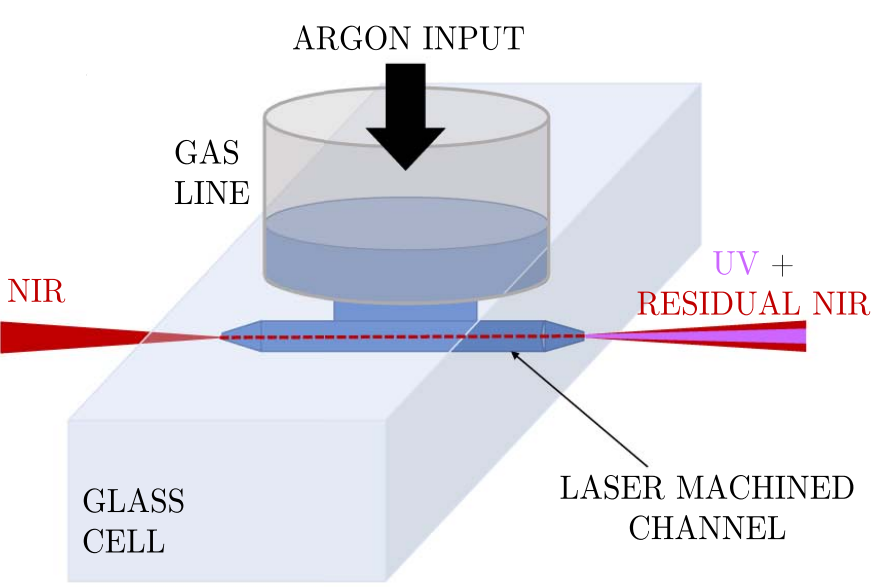
\includegraphics[width=\textwidth]{im/schematic_galli}
   \caption{}\label{im:thg_schematic}
    \end{subfigure}  
 \begin{subfigure}{0.5\textwidth}
        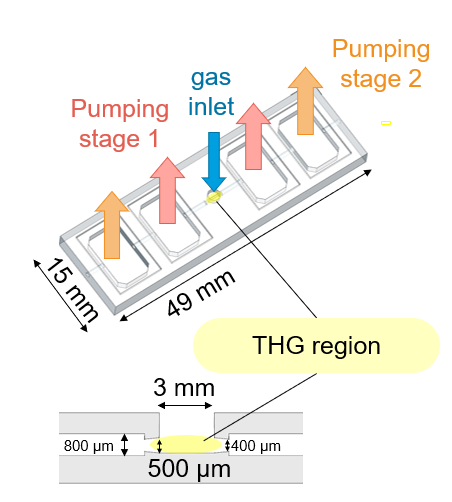
\includegraphics[width=\textwidth]{im/new_chip_edited}
    \caption{}\label{im:new_chip}
    \end{subfigure}
\caption{The fused silica chip used to confine the gas for THG. 
Figure \ref{im:thg_schematic}, reproduced from \cite{galli2019}, shows a simplified schematic of the THG process taking place in the glass cell, without the pumping system, while Figure \ref{im:new_chip}, reproduced from Josina Hahne's master's thesis defence, gives a detailed overview of the chip's design.}
\end{figure}
The CFEL-ATTO group generates few-femtosecond UV laser pulses via THG in a gas cell. This is driven by a pulsed near-infrared (NIR) Ti:sapphire laser with a central wavelength of 800nm and a repetition rate of 1kHz. Self-phase modulation in a hollow-core fibre filled with a gradient of helium gas, followed by subsequent compression via chirp mirrors is used to produce NIR pulses with a duration of around 5fs and a pulse energy of up to 3mJ. A fraction of the NIR beam is focussed into a vacuum chamber for UV generation, resulting in a spatially approximately Gaussian beam with a 1/$e^2$ beam waist of 65$\mu$m. The chamber contains a glass chip made of fused silica (SiO$_2$), a gas inlet and a pumping system. Its specifications are central to the THG process and are described in more detail in the following. \par 
The fused silica chip is equipped with a laser machined central 3mm-long channel with a 0.5mm diameter at the centre, gradually reducing to 400 microns at the extremities. Pressurised gas, normally Argon or Neon, is pumped through the channel, with a two-stage differential pumping system on both sides of the 3mm central interaction region ensuring a tight confinement of the gas in this region. As the pump beam passes through the cell and interacts with the pressurised gas THG takes place, which results in UV pulses being generated. The UV components are then separated from the pump beam upon exiting the vacuum chamber via dichroic mirrors, which reflect in the UV but transmit in the NIR. Figure \ref{im:thg_schematic} shows a simplified schematic of this set-up, without the pumping system. The fused silica chip, including the two pumping stages, is shown in Figure \ref{im:new_chip}, with the 3mm central interaction region highlighted. \par 
The fused silica chip shown in Figure \ref{im:new_chip} is an improved design on a simpler  cell which was used previously, such as in \cite{galli2019}. The old and new cell have the same 3mm central interaction region but differ in their implementation of the pumping system.   Note that all measurements presented in this report were taken with the new chip in place. 

\section{Simulation Results and Discussion}
In order to reproduce the experimental conditions described above as closely as possible, the simulation input was largely based on measured data. Thus, the time-frequency information as well as the central wavelength of the NIR input pulse used to model the pump beam in the simulations were read in from experimental data. Spatially, the input beam was assumed to be a Gaussian with a beam waist and focus position corresponding to the values found experimentally. \par 
Apart from the profile of the NIR input beam, the most important THG condition to be modelled was the gas density distribution in the fused silica chip. A fully realistic model of the gas distribution, taking into account the geometry of the chip as well as the effects of the differential pumping system, is challenging to obtain. Some efforts to achieve this have been made using the \textit{COMSOL Multiphysics} software but no sufficiently accurate model of the gas distribution throughout the entire chip could be produced at this point. Therefore, the THG simulations presented here focus exclusively on the 3mm central interaction region of the chip. The density distribution in this region was modelled using a gradient profile, based on the central pressure at the gas inlet and the pressure at the edges of the central interaction region, which has been measured to be around 1mbar. The gradient model is based on an interpolation of pressure values between the central and the edge pressure using the equation 
\begin{equation}
p(z)^2 = p(z_0)^2 + (z-z_0) \frac{p(z_1)^2 - p(z_0)^2}{z_1 - z_0}, 
\end{equation}
where $p$ is pressure and $z$ is a point between $z_0$ and $z_1$, two points at which the pressure is known, such as the centre and edges of the THG region. The density distribution is then inferred from the interpolated pressure distribution. Figure \ref{im:grad} shows the resulting density model for different central pressures. \par 
\begin{figure}[h]
\centering
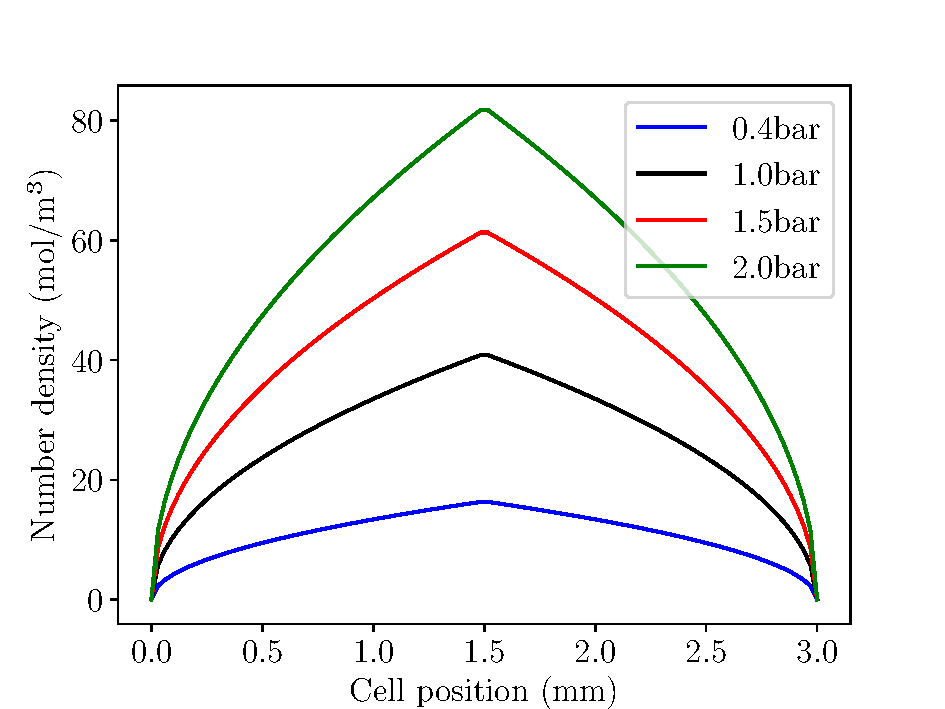
\includegraphics[width=0.5\textwidth]{im/grad_model}
\caption{Gas densities in the central interaction region of the gas cell for different central pressures using the gradient model.}\label{im:grad}
\end{figure} 
While discrepancies between this simplified density model and the real distribution are to be expected, especially due to the lower-density regions just outside the cell in which relevant pulse-shaping and absorption processes likely take place being ignored, the gradient model can provide qualitatively meaningful results. \par 
The simulations can be run for a variety of different gases, central pressures and input beam powers but the results presented in this report will, for concision, mostly focus on Argon at 150mW NIR power and Neon at 400mW NIR power, with central gas pressures of 0.4bar and 2.0bar, respectively. These values were chosen due to the availability of high-quality experimental data at these parameters. 

\subsection{Comparison with Experiment}
The most important metric when evaluating the performance of the simulations is a comparison with experimental data. \par 
It is important to point out that in order to allow for a direct comparison between simulated and measured data the pressure values for the simulated data were rescaled by an empirically determined factor of 2.5. This mismatch in pressure scales has a physical origin beyond the shortcomings of the gradient model: measuring the absolute gas pressure value in the central interaction region is an experimental challenge and hence the pressure set for the gas inlet is taken as a proxy for the central pressure. Thus, when taking UV output data at some central pressure in the gas cell, the recorded pressure  might only approximately correspond to the actual central pressure. Since the simulations are based directly on pressures in the central interaction region, their pressure values must be rescaled to take into account this systematic error when comparing with measured data. Throughout this report, simulated data will therefore always be presented using rescaled pressure. \par 
\begin{figure}[h]
\centering
 \begin{subfigure}{0.5\textwidth}
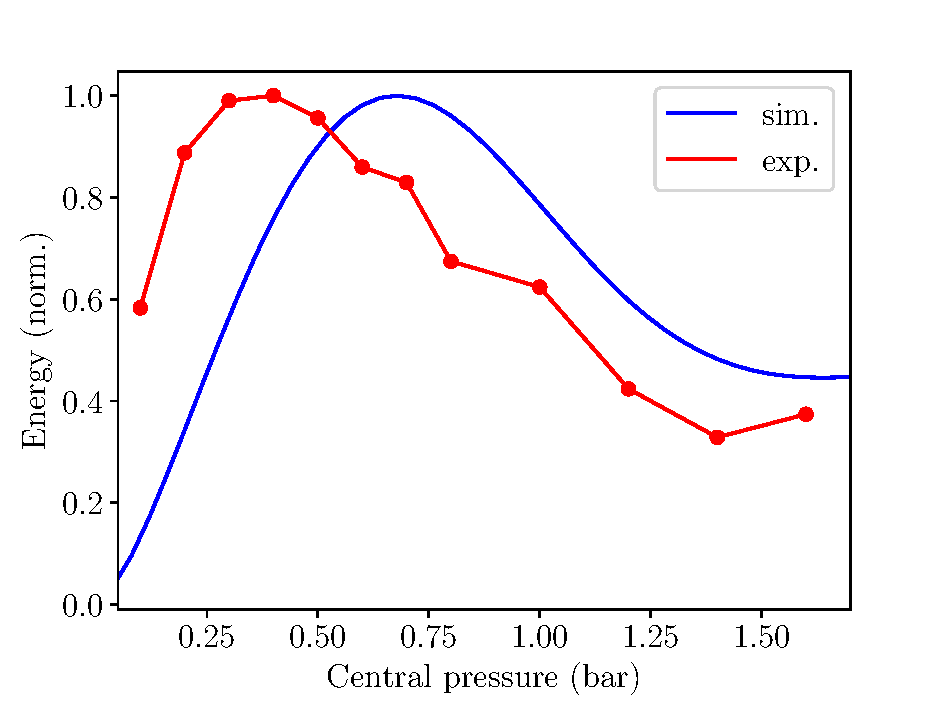
\includegraphics[width=\textwidth]{im/energies_Ar}
\caption{Argon at 150mW NIR beam power}\label{im:sim_v_measured_Ar}
\end{subfigure}
 \begin{subfigure}{0.5\textwidth}
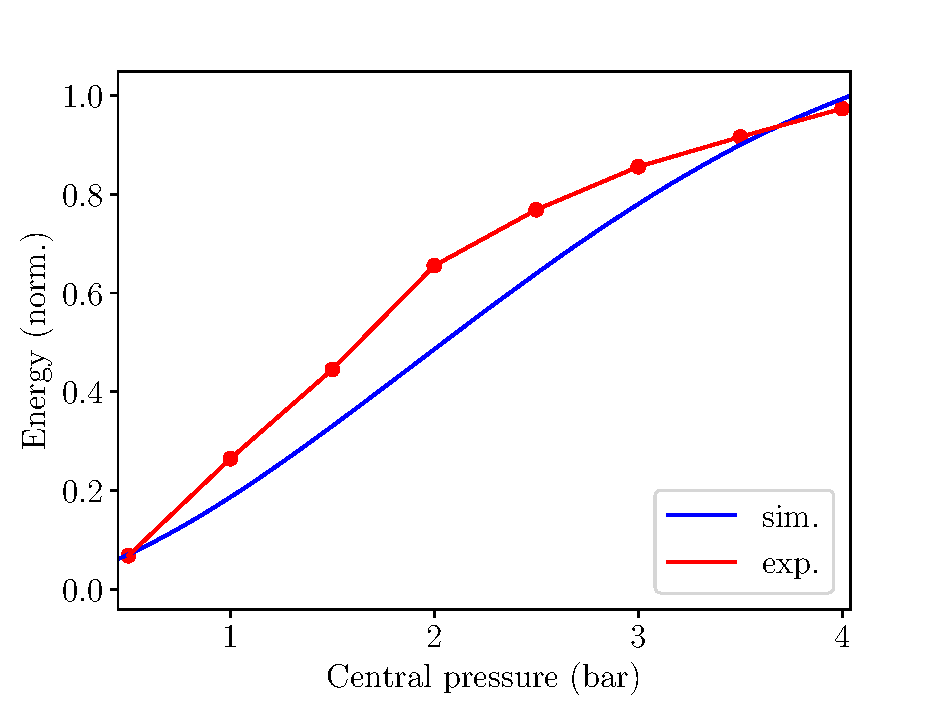
\includegraphics[width=\textwidth]{im/energies_Ne}
\caption{Neon at 400mW NIR beam power}\label{im:sim_v_measured_Ne}
\end{subfigure}
\caption{Simulated and experimental values of normalised UV output energies at different (rescaled) central pressures.}\label{im:sim_v_measured}
\end{figure}
Figure \ref{im:sim_v_measured} shows simulated and measured UV output energies at various (rescaled) central pressures for both Argon and Neon. The energy axes of the plots are normalised to allow for a better qualitative comparison despite a discrepancy between the simulated and measured energies by a factor of roughly ten. This overestimation of the UV energies in the simulations can likely be attributed to the simplistic gas density distribution used, which does not take into account absorption and other effects in the low-density regions outside the central interaction region. As can be seen, there is good qualitative agreement between the simulated and measured UV output pulse energies for both Argon and Neon: the simulations can clearly reproduce general trends concerning the relationship between UV energies and gas pressure, even when using the simplified gradient model. \par 
While the simulated energy-pressure function for Argon captures the shape of the measured data well, it is offset by a pressure value of roughly 0.3bar. For Neon, no such offset is apparent, though the normalised energy-pressure curve is reproduced less accurately.   Both of these effects can be adjusted for, resulting in significantly better agreement between simulations and experiment, by using different pressure scaling factors for the two gases, accounting for the fact that they are measured in different pressure regimes. It is unclear whether this step could be justified with respect to physical consistency, however. \par 
Figure \ref{im:sim_v_measured} shows that in both simulations and experiment, UV energies (initially) rise with increasing central pressure. This is due to higher pressures being associated with higher gas densities in the cell and hence the presence of more polarisable gas atoms. Thus, the total nonlinear polarisation response is increased and more THG takes place. At higher pressures, the trend slows down and eventually reverses because of ionisation effects: the UV beam in the gas cell becomes sufficiently intense to contribute to the ionisation of the gas atoms, resulting in a depleted output beam. Saturation sets in more quickly for Argon than for Neon due to its ionisation potential being lower and its $\chi^{(3)}$ value being higher. Note that while no Neon saturation can be seen in Figure \ref{im:sim_v_measured}, it has been observed experimentally at higher pressures.  \par 
\begin{figure}[h]
\centering
 \begin{subfigure}{0.5\textwidth}
\includegraphics[width=\textwidth]{im/spec_comp_Ar_150mw_2.5scale_0.4bar}
\caption{Argon at 150mW and 0.4bar}\label{im:spec_Ar}
\end{subfigure}
 \begin{subfigure}{0.5\textwidth}
\includegraphics[width=\textwidth]{im/spec_comp_Ne_400mw_2.5scale_2.0bar}
\caption{Neon at 400mW and 2.0bar}\label{im:spec_Ne}
\end{subfigure}
\caption{Simulated and measured UV output spectra. The power values in the subfigure captions refer to the NIR beam power and the pressure values to the (rescaled) central cell pressures.}\label{im:spec}
\end{figure}
Beyond the UV energies, it is also instructive to consider the simulated UV output spectra. Figure \ref{im:spec} compares the measured and simulated spectra for both Argon and Neon. Despite the simplicity of the gradient model, the simulated spectra are fairly accurate, with the general features of the experimental spectra being reproduced clearly. As expected, the spectra are centred on roughly 266nm, corresponding to the third harmonic of the central wavelength (800nm) of the NIR input beam. \par  
\begin{figure*}[h]
\centering
 \begin{subfigure}{0.49\textwidth}
        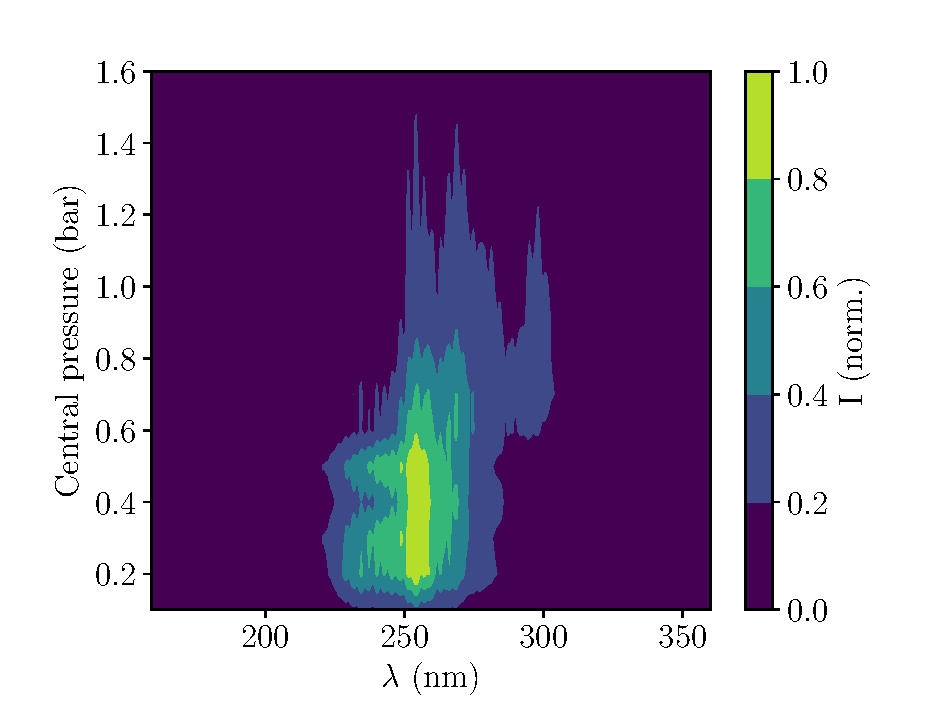
\includegraphics[width=\textwidth]{im/2d_spectra_pres_Ar_150mW_meas}
    \caption{Argon (measured)}
    \end{subfigure}
    \begin{subfigure}{0.49\textwidth}
        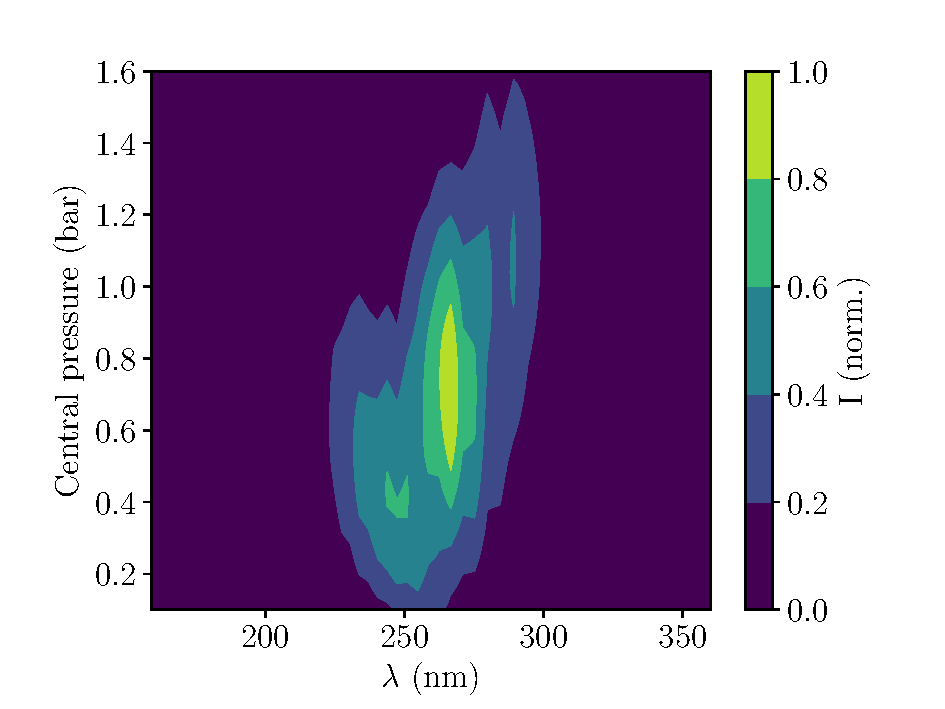
\includegraphics[width=\textwidth]{im/2d_Ar_sim}
    \caption{Argon (simulated)}
    \end{subfigure}   
     \begin{subfigure}{0.49\textwidth}
        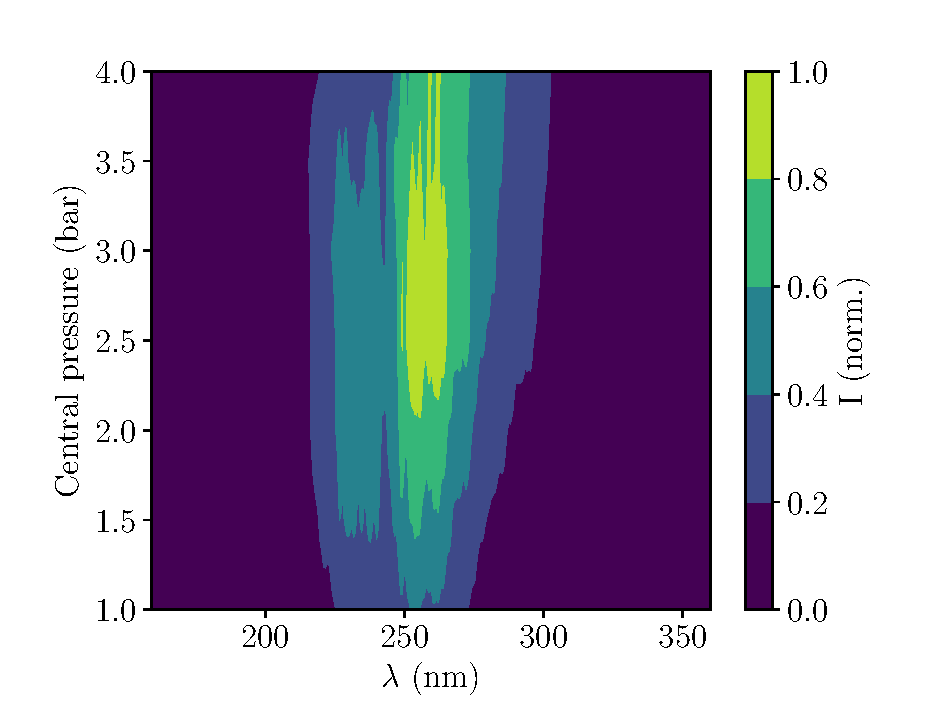
\includegraphics[width=\textwidth]{im/2d_spectra_pres_Ne_400mW_meas}
    \caption{Neon (measured)}
    \end{subfigure}
    \begin{subfigure}{0.49\textwidth}
        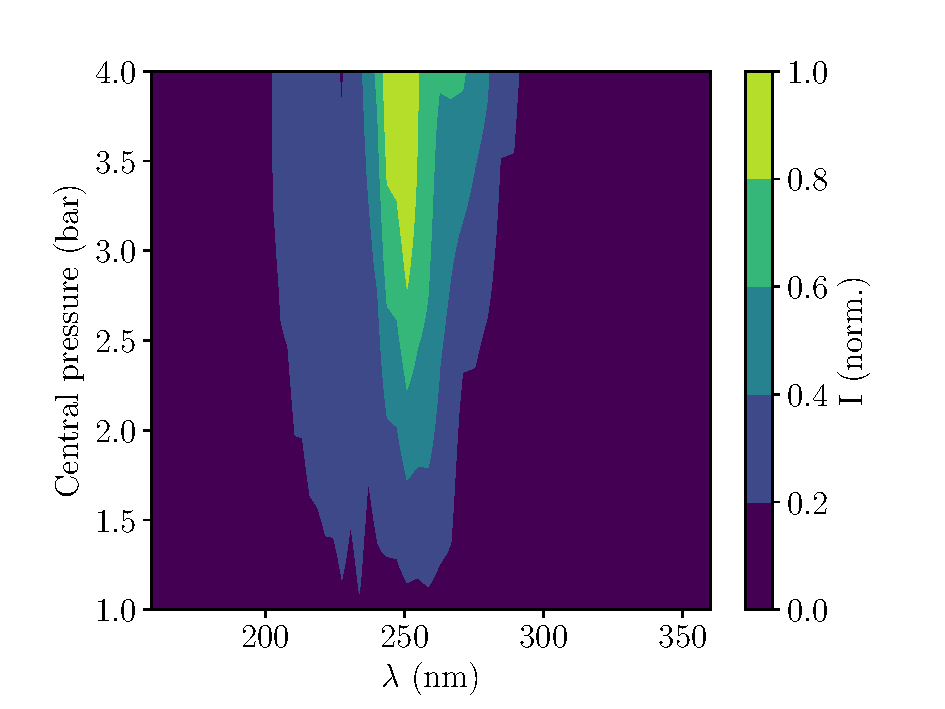
\includegraphics[width=\textwidth]{im/2d_Ne_sim}
    \caption{Neon (simulated)}
    \end{subfigure}  
\caption{UV output spectra at different (rescaled) central pressures. The top row corresponds to Argon at 150mW NIR power while the bottom row corresponds to Neon at 400mW NIR power}\label{im:spec_2d}
\end{figure*}
A comparison of simulated and experimental UV spectra across different (rescaled) central pressures is shown in Figure \ref{im:spec_2d}. For Argon, the simulations reproduce the general trend of a gradual red-shift with increasing pressures as well as a decrease in spectral intensity due to saturation at high pressures. However, due to the same pressure offset mentioned when discussing Figure \ref{im:sim_v_measured_Ar}, there is a mismatch with respect to when these effects set in, despite the pressure rescaling. For Neon, the general shape of the simulated intensity contour matches that of the experimental data, although the measured saturation of the spectral intensity is not reproduced in the simulations. Note that the fact that the measured Neon spectra have their most intense peaks between roughly 2.5 and 3.5bar and then decrease in intensity is not in contradiction to no comparable UV energy peak being observed at these pressures, as was seen in Figure \ref{im:sim_v_measured_Ne}. This is due to the UV energy being represented by the integral of the spectral intensity across the UV spectrum, so that the effect of a lower peak spectral intensity on the resulting total UV energy is compensated by a broadening of the spectrum.  \par 
In summary, despite the simplified gradient model used to describe the gas density distribution in the central interaction region, the simulations were able to qualitatively reproduce important features and trends of the experimental data. 

\subsection{Self-defocusing and Ionisation}
Having demonstrated that the simulations, even at their present stage, can produce output in reasonable agreement with experimental data, it is now worth considering applications of the simulations beyond reproducing measured values. An important application of the simulations is gaining information about UV pulse properties that are difficult to access experimentally. While this is a broad aim, the following section focusses on self-defocusing effects as a case study. For concision, only Argon is considered, although similar results can be observed for Neon. \par  
\begin{figure}[H]
\centering
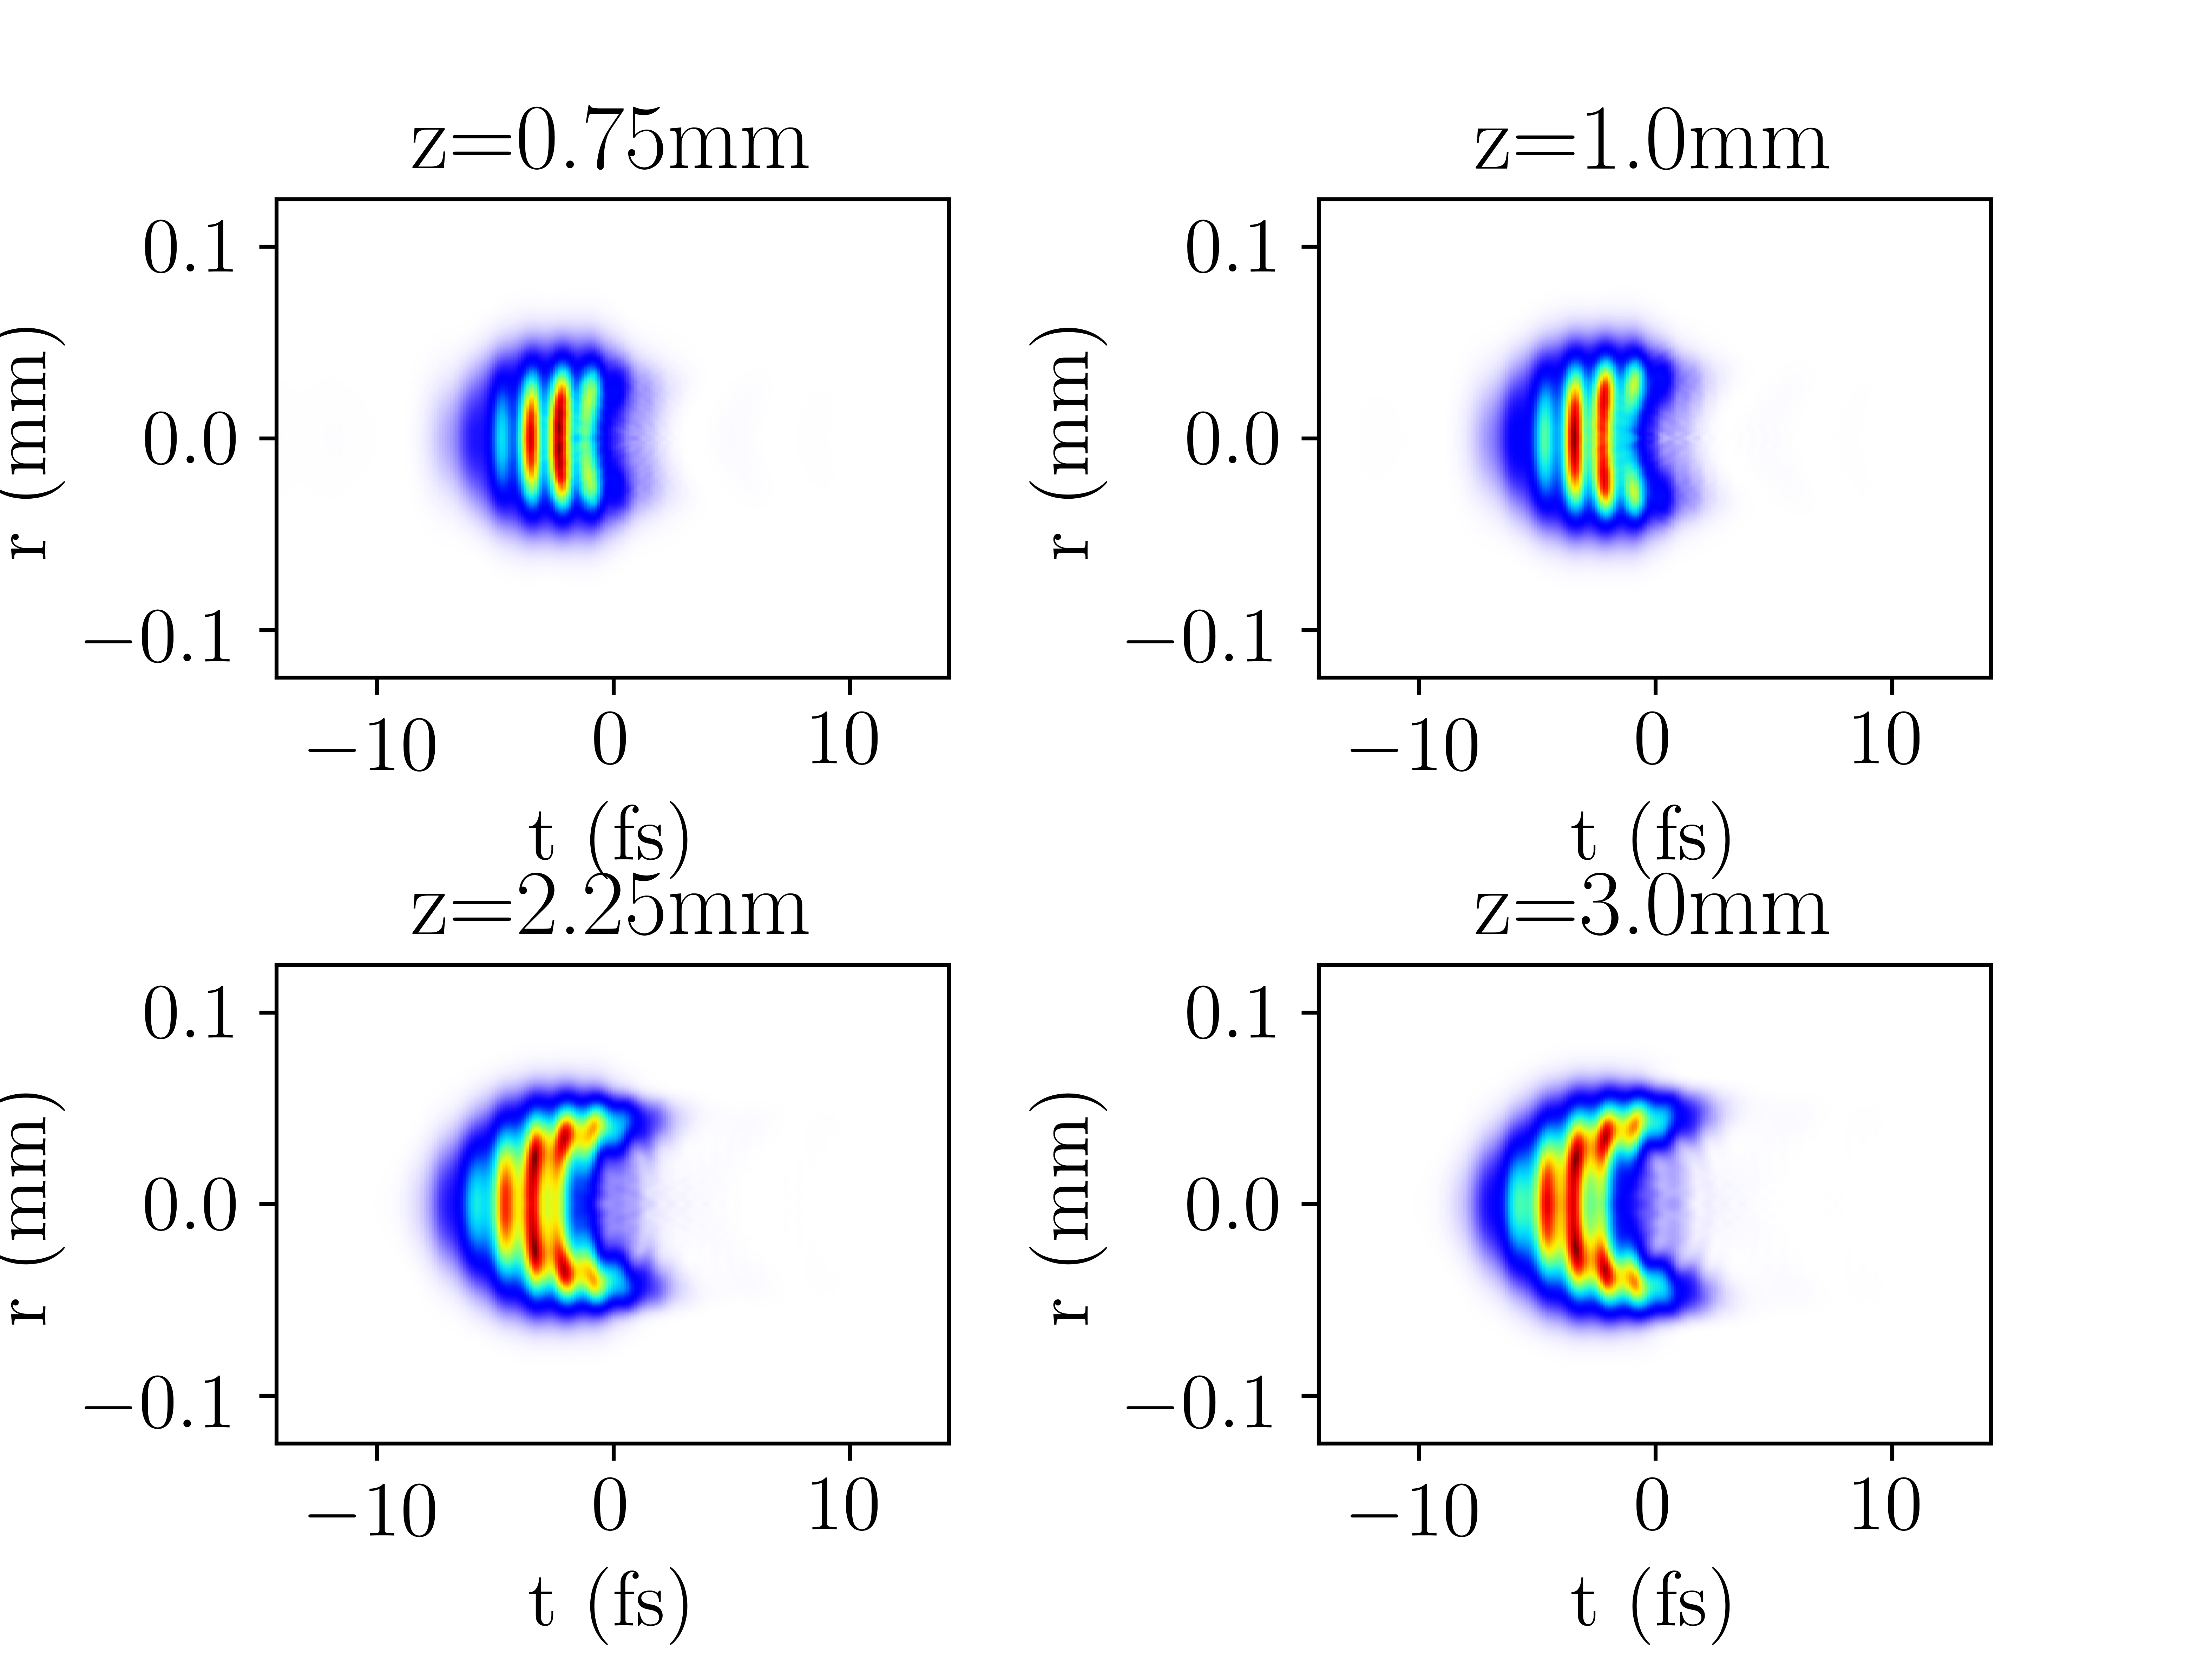
\includegraphics[width=0.5\textwidth]{im/UV_pulse_evolution_Ar_ion}
\caption{Simulated spatiotemporal beam profiles of the UV pulses at various locations in the 3mm gas cell. Argon at 150mW NIR power and 0.4bar (rescaled) central pressure is used.}\label{im:prop}

\end{figure}
\begin{figure*}[h]
\centering
 \begin{subfigure}{0.49\textwidth}
        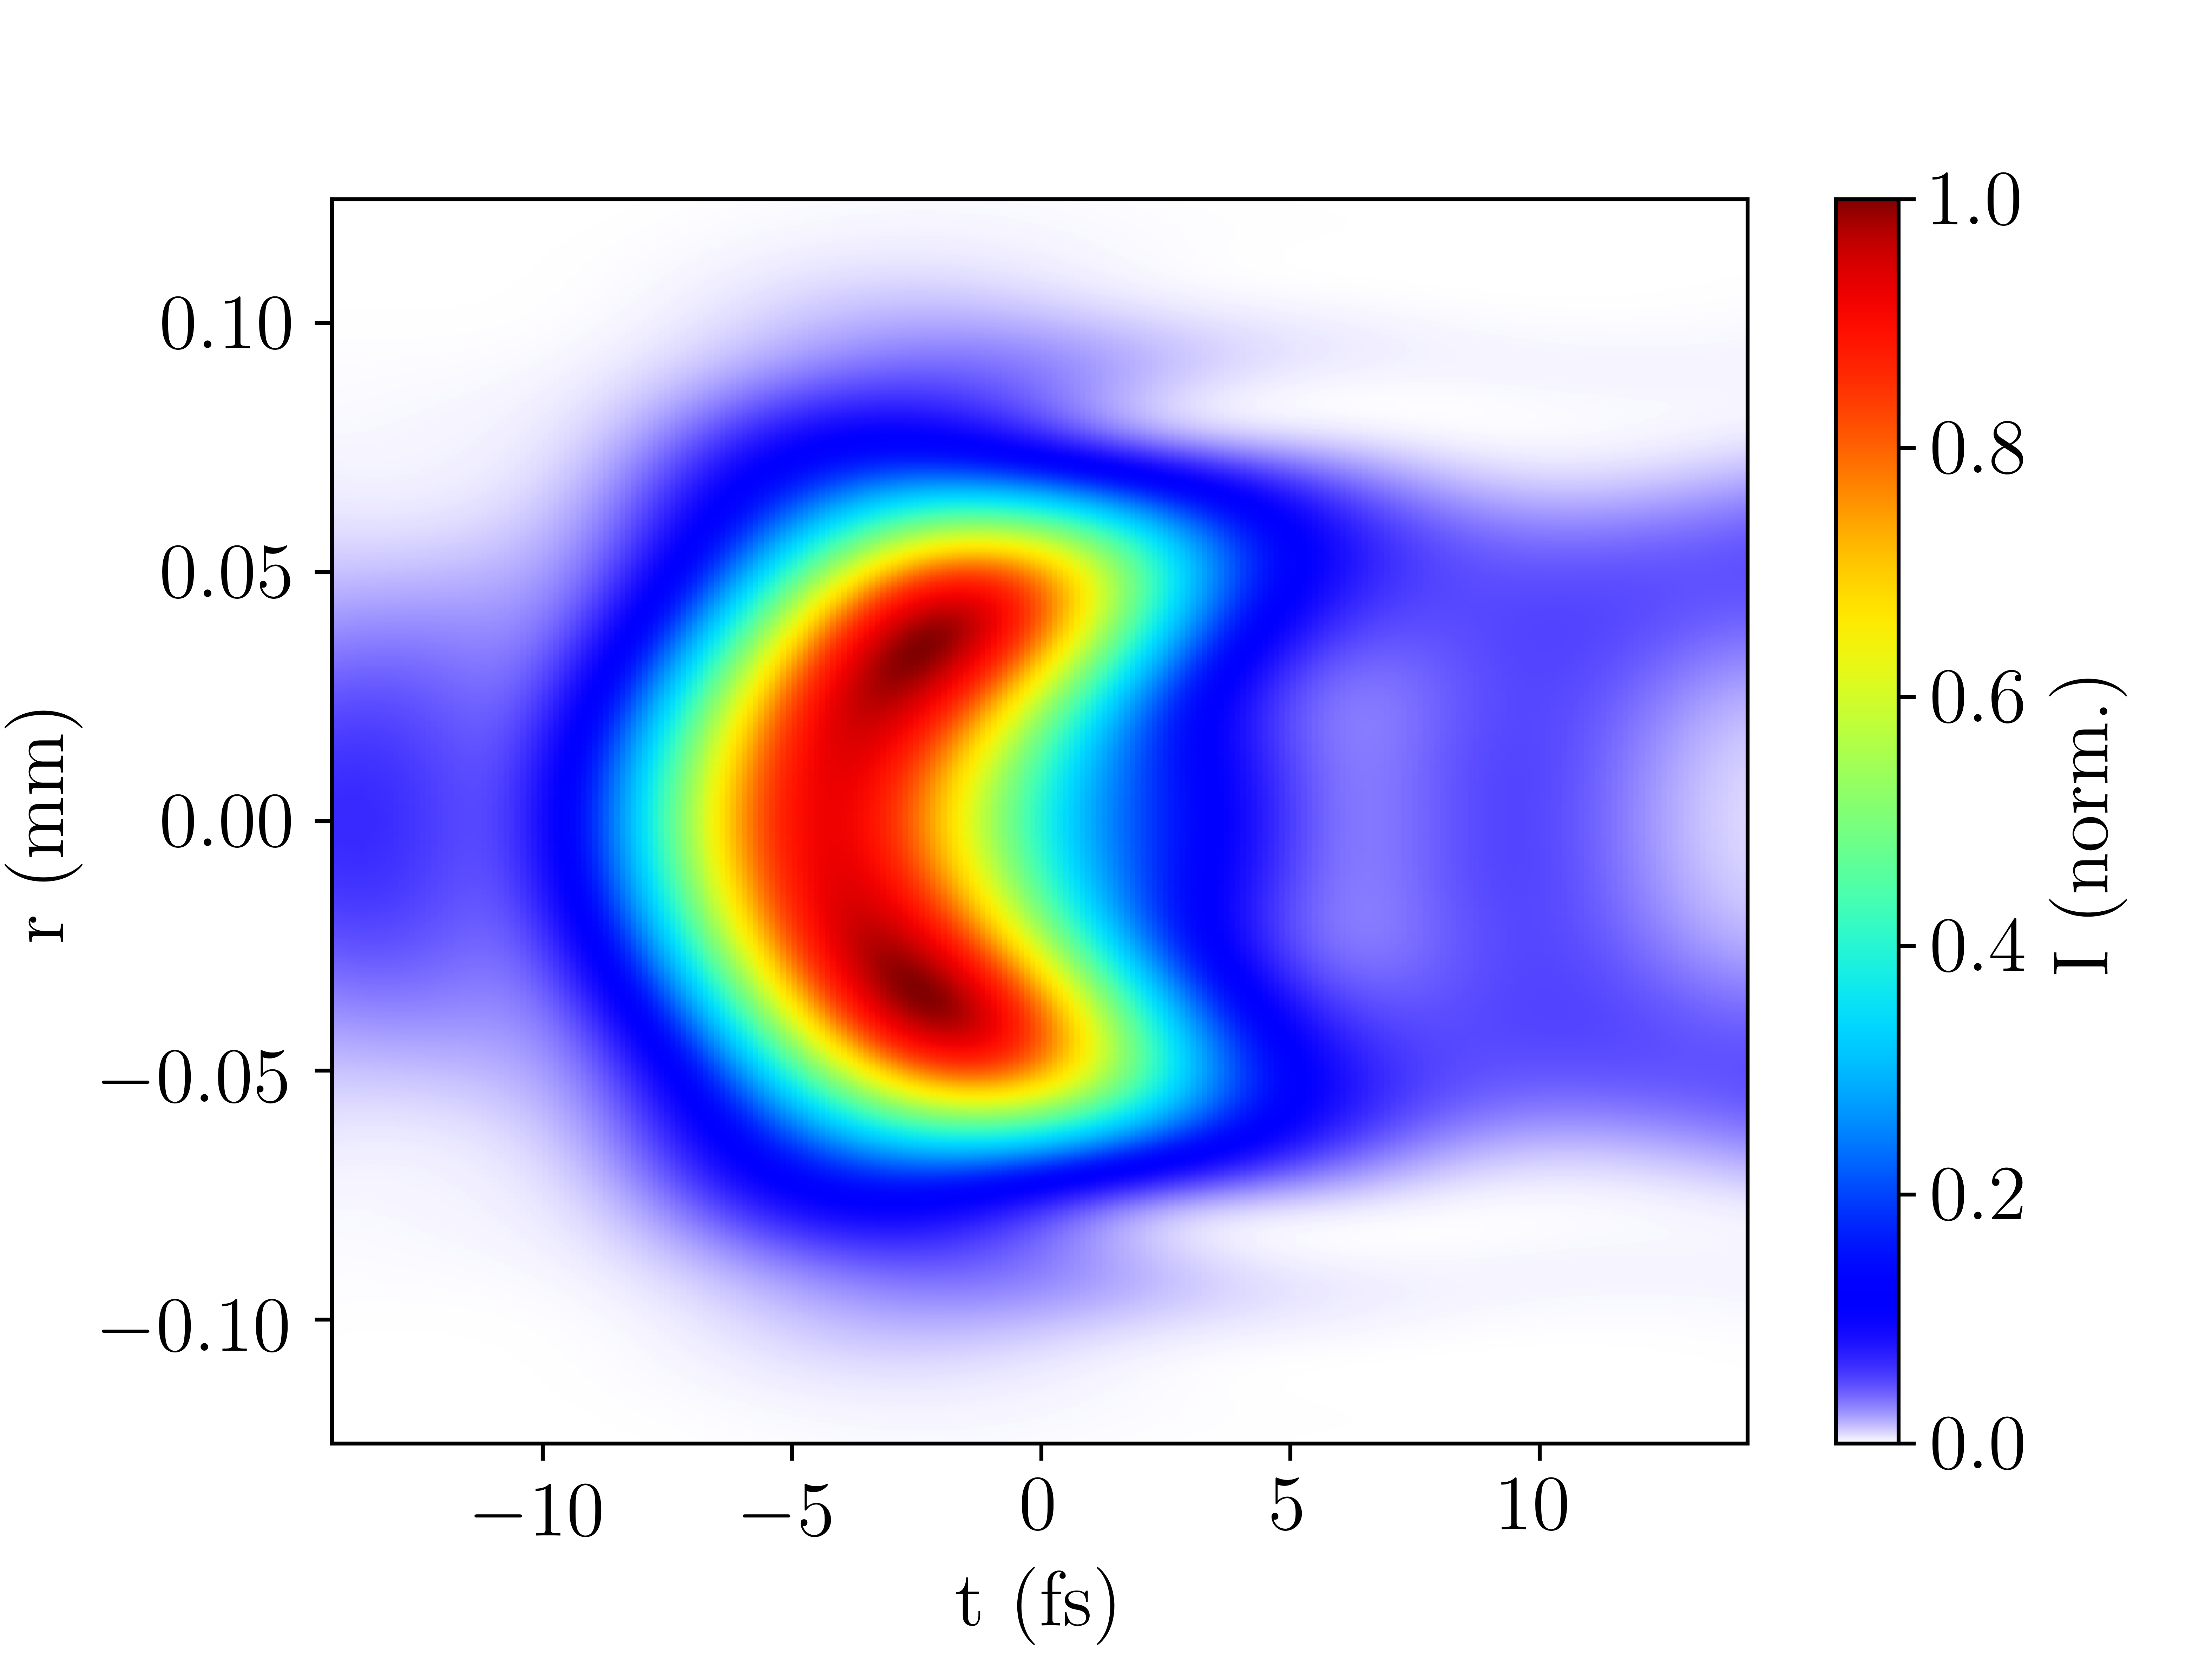
\includegraphics[width=\textwidth]{im/IR_pulse_output_Ar_ion}
    \caption{NIR beam with ionisation}
    \end{subfigure}
    \begin{subfigure}{0.49\textwidth}
        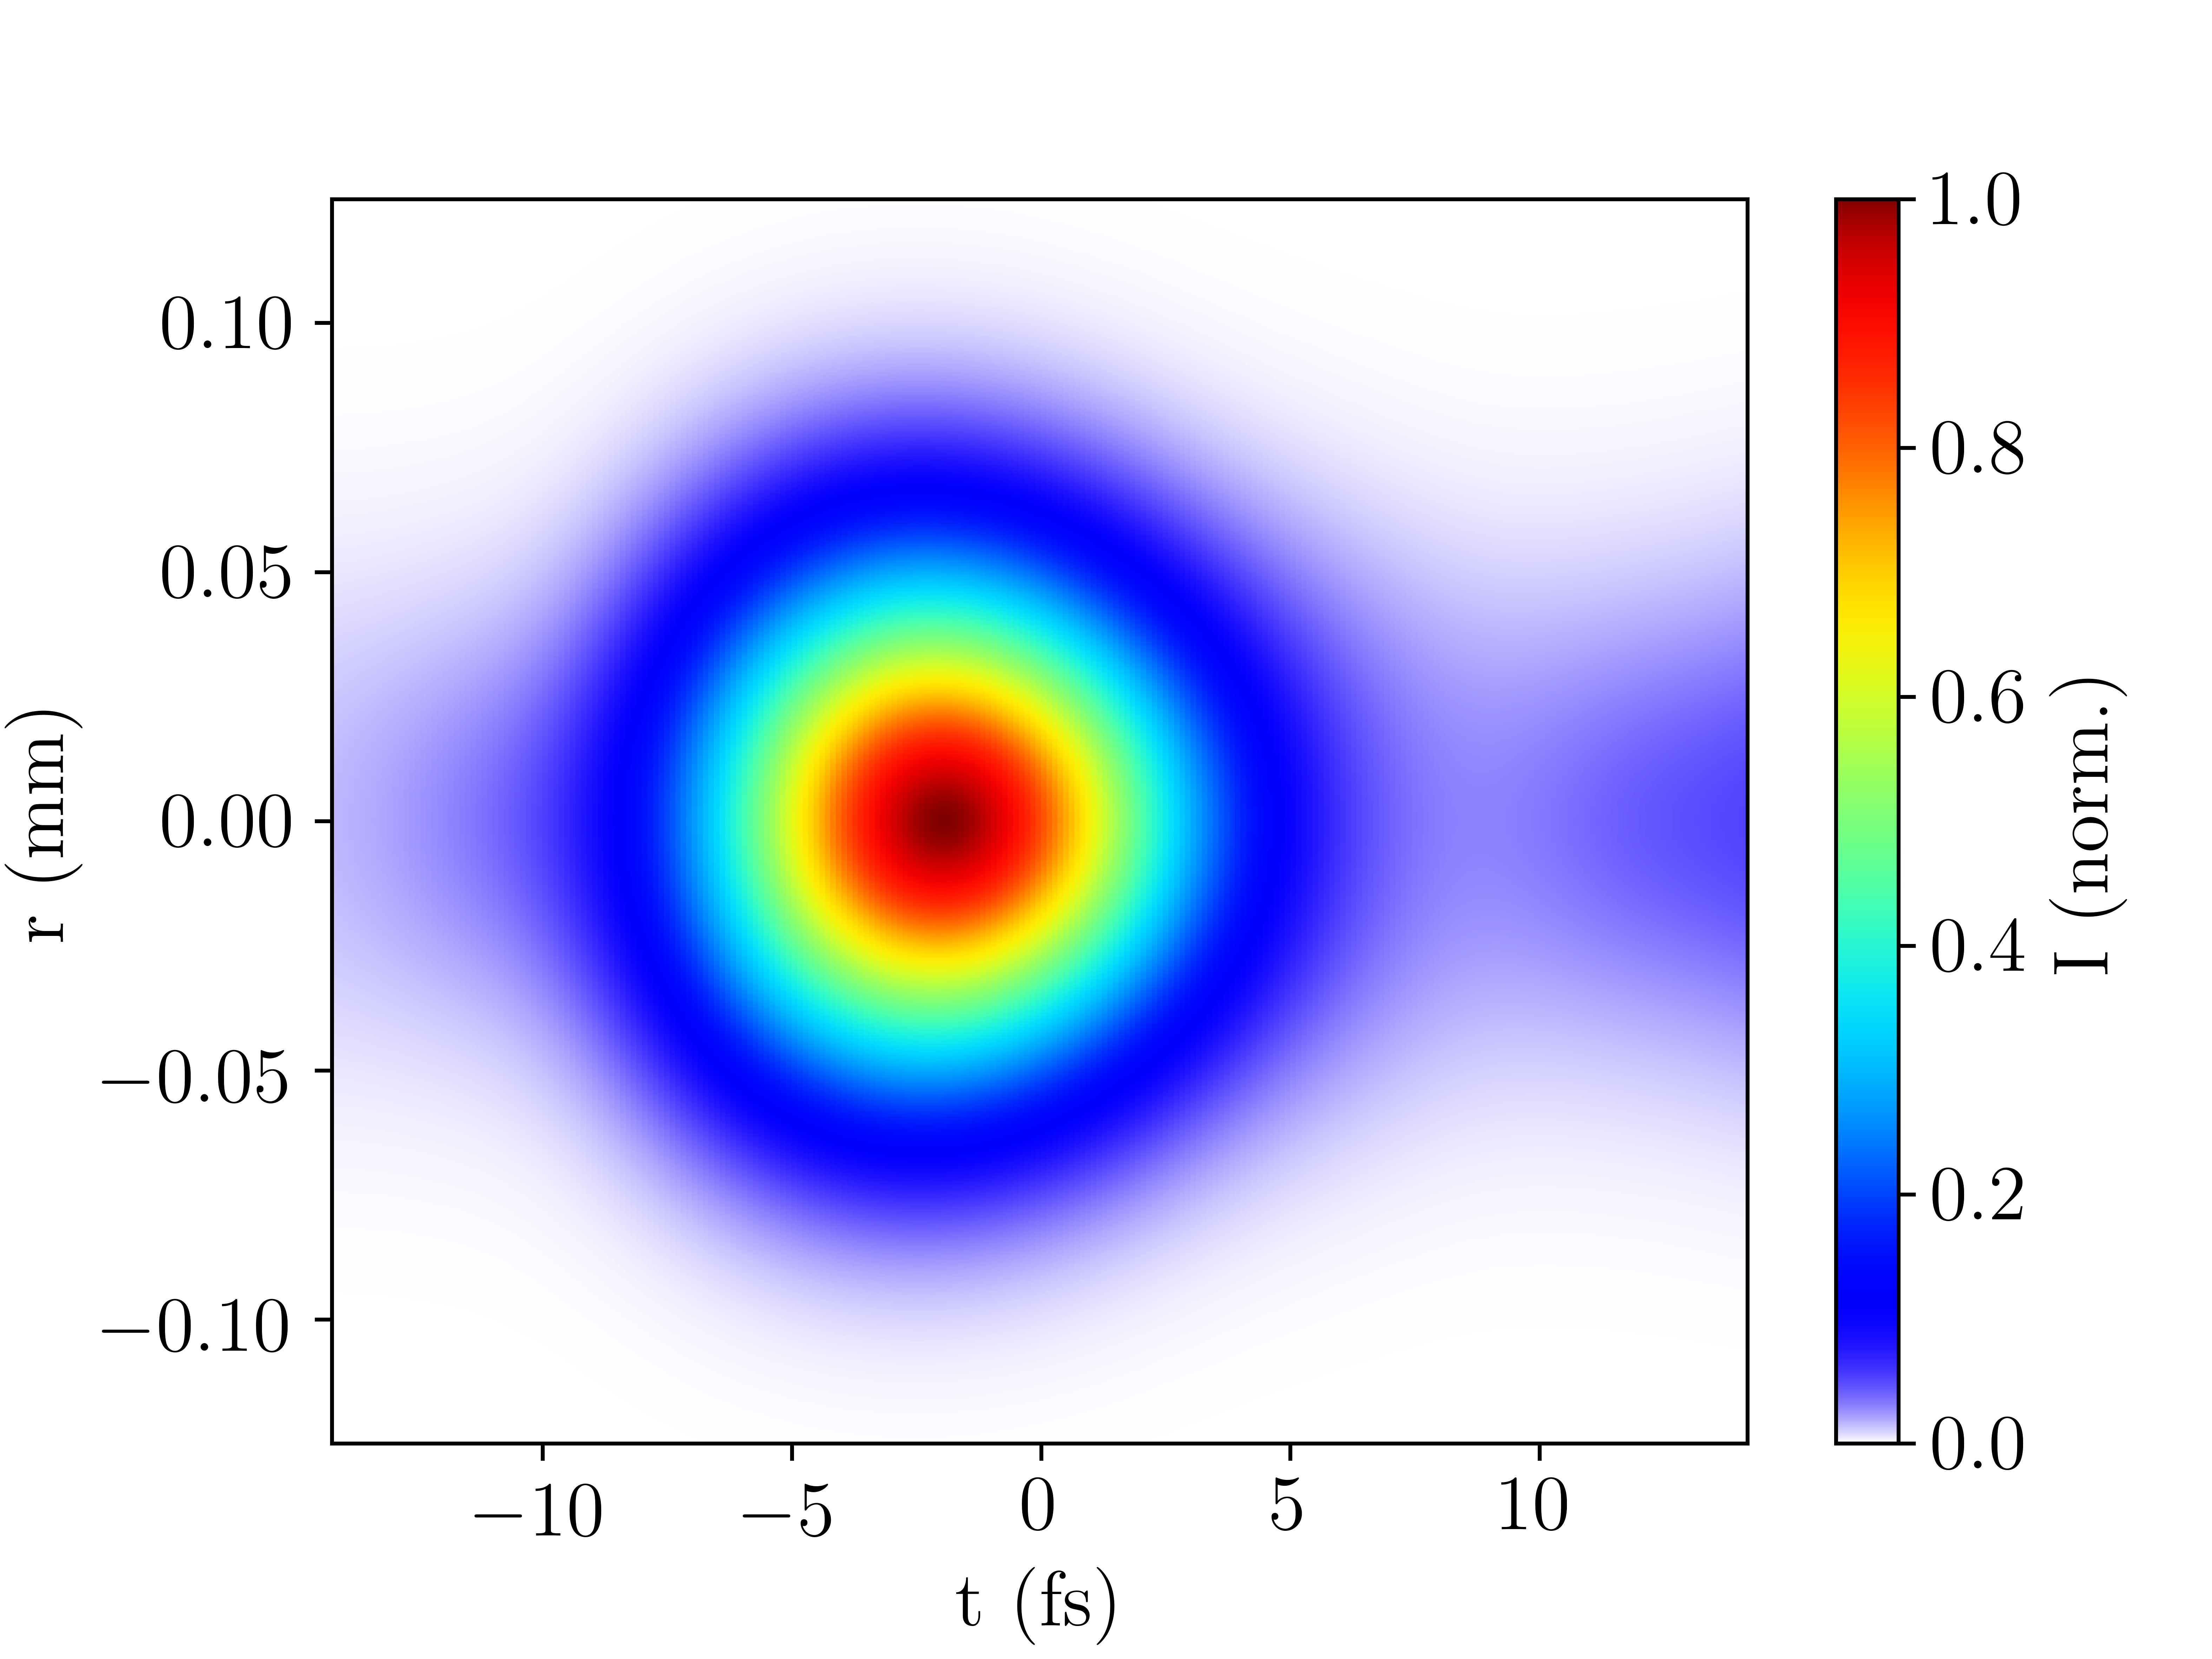
\includegraphics[width=\textwidth]{im/IR_pulse_output_Ar_no_ion}
    \caption{NIR beam without ionisation}
    \end{subfigure} 
    \begin{subfigure}{0.49\textwidth}
        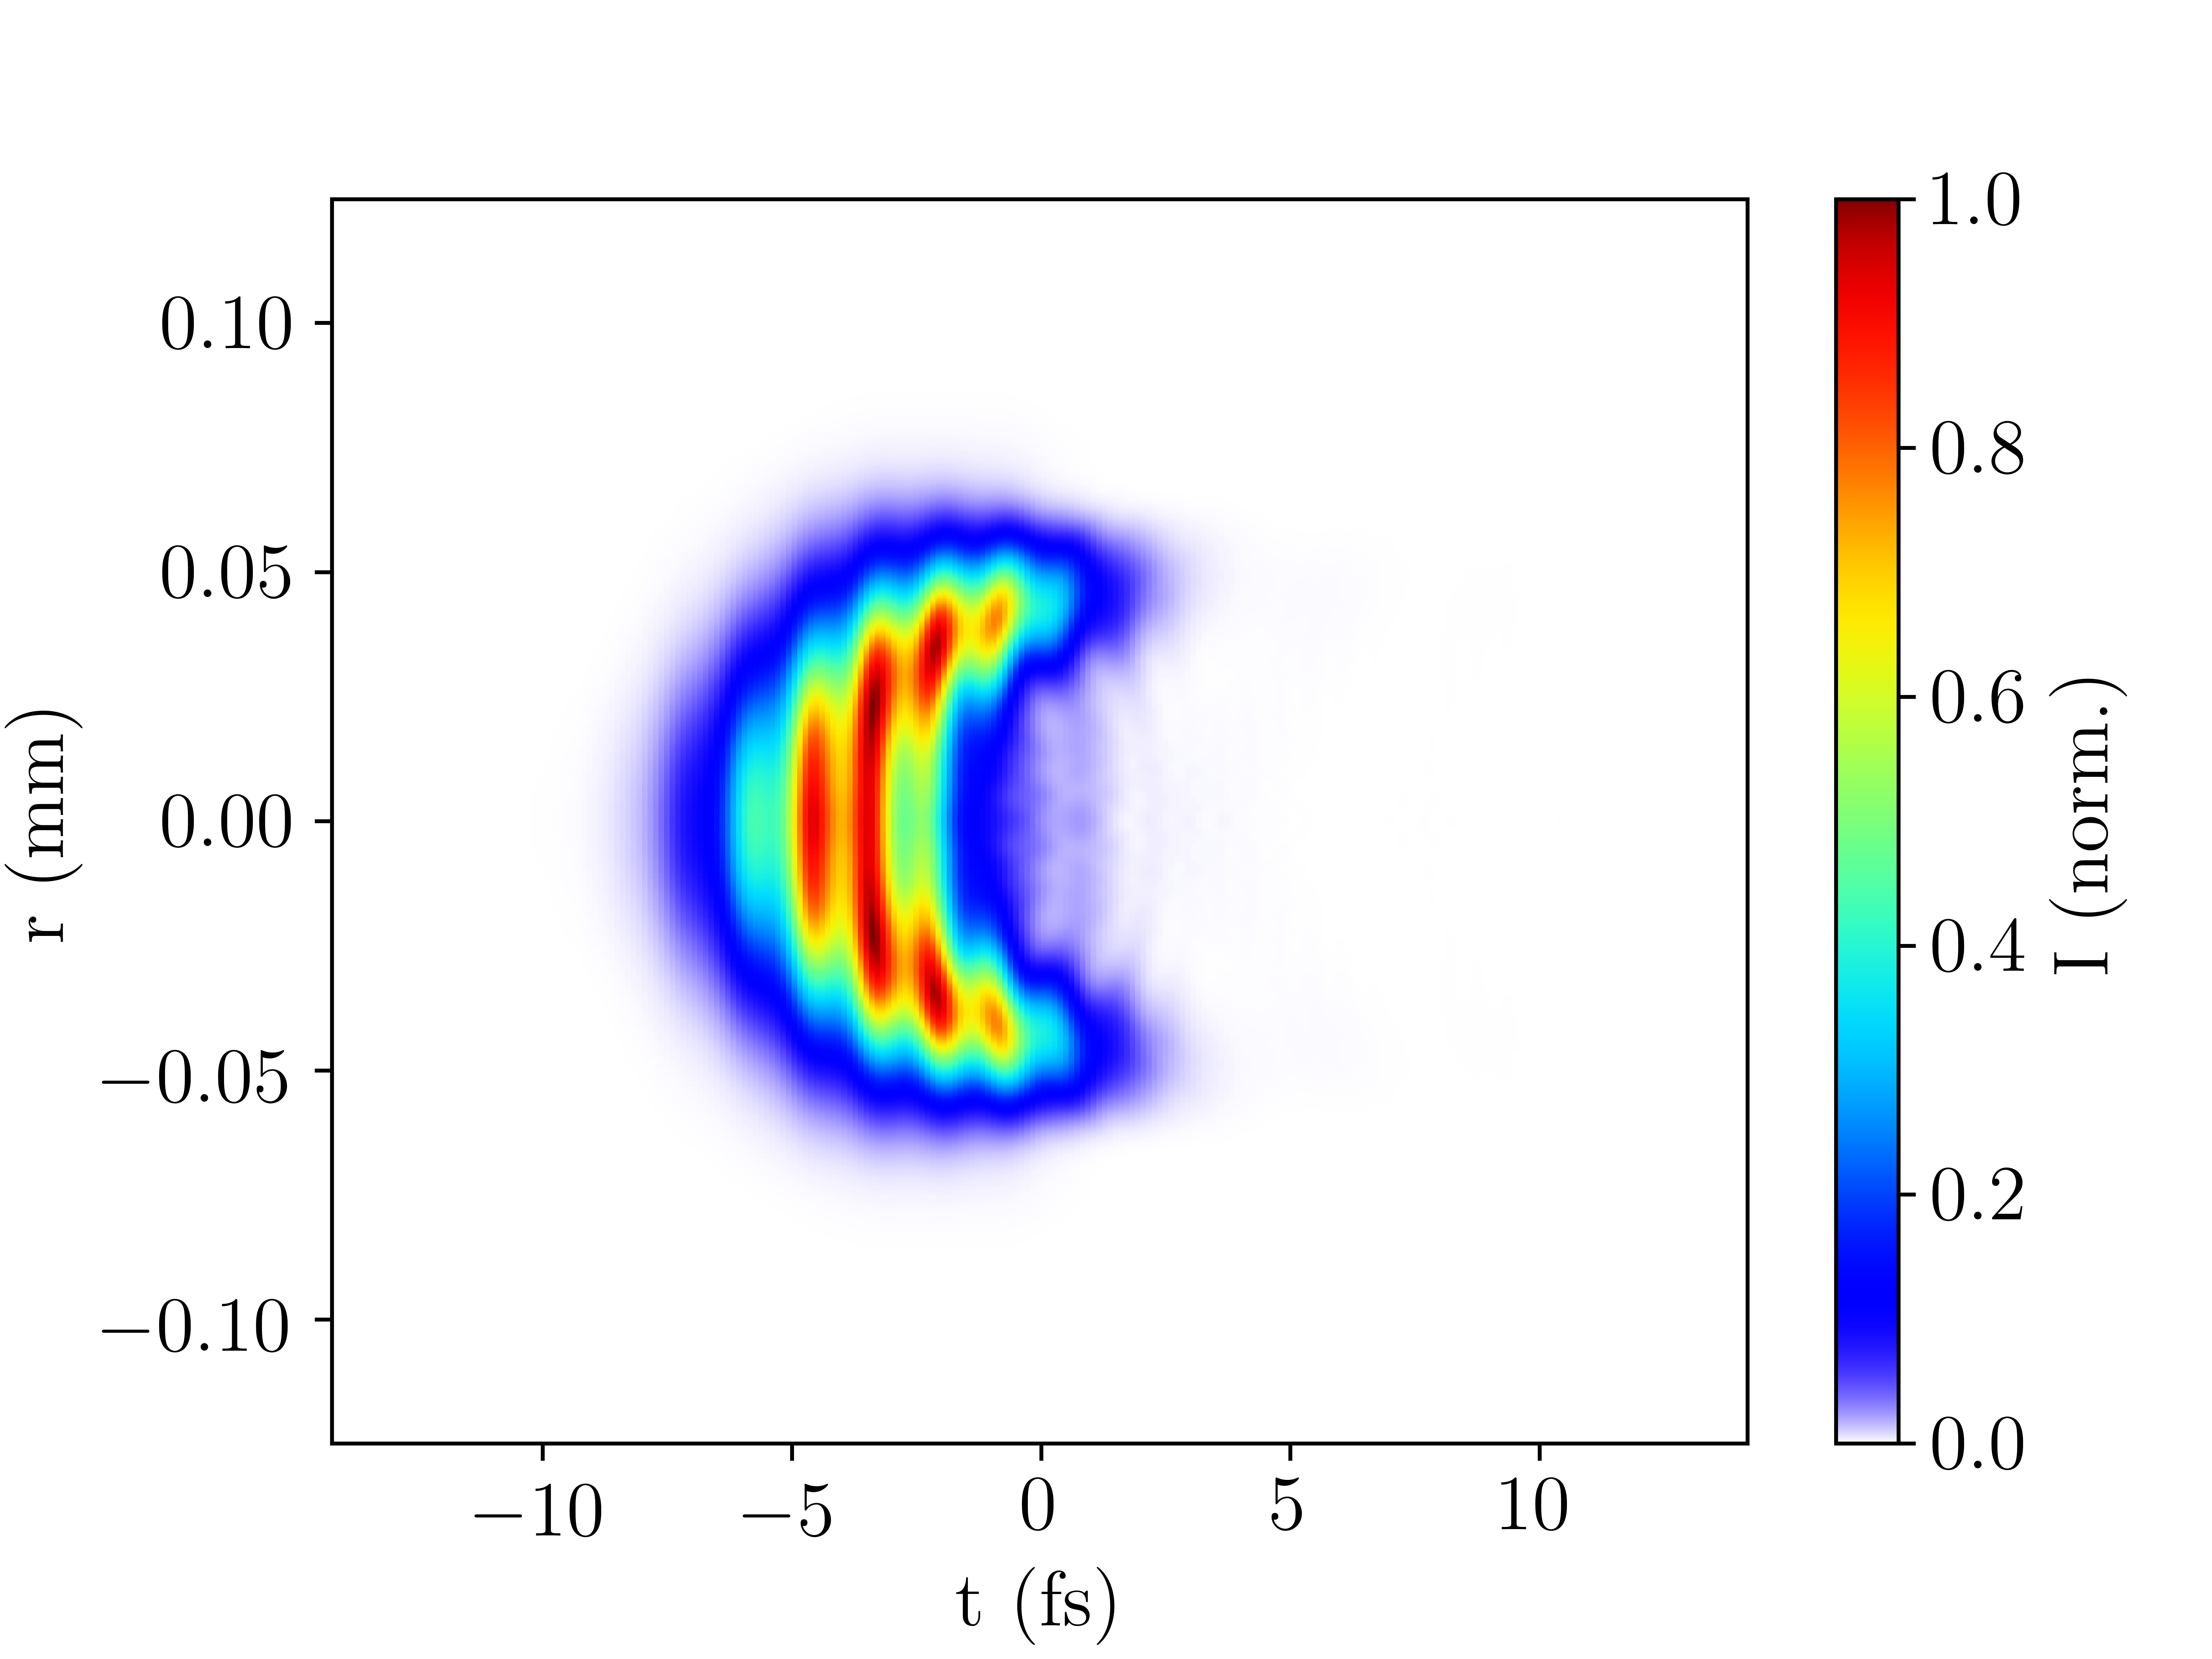
\includegraphics[width=\textwidth]{im/UV_pulse_output_Ar_ion}
    \caption{UV beam with ionisation}
    \end{subfigure}
    \begin{subfigure}{0.49\textwidth}
        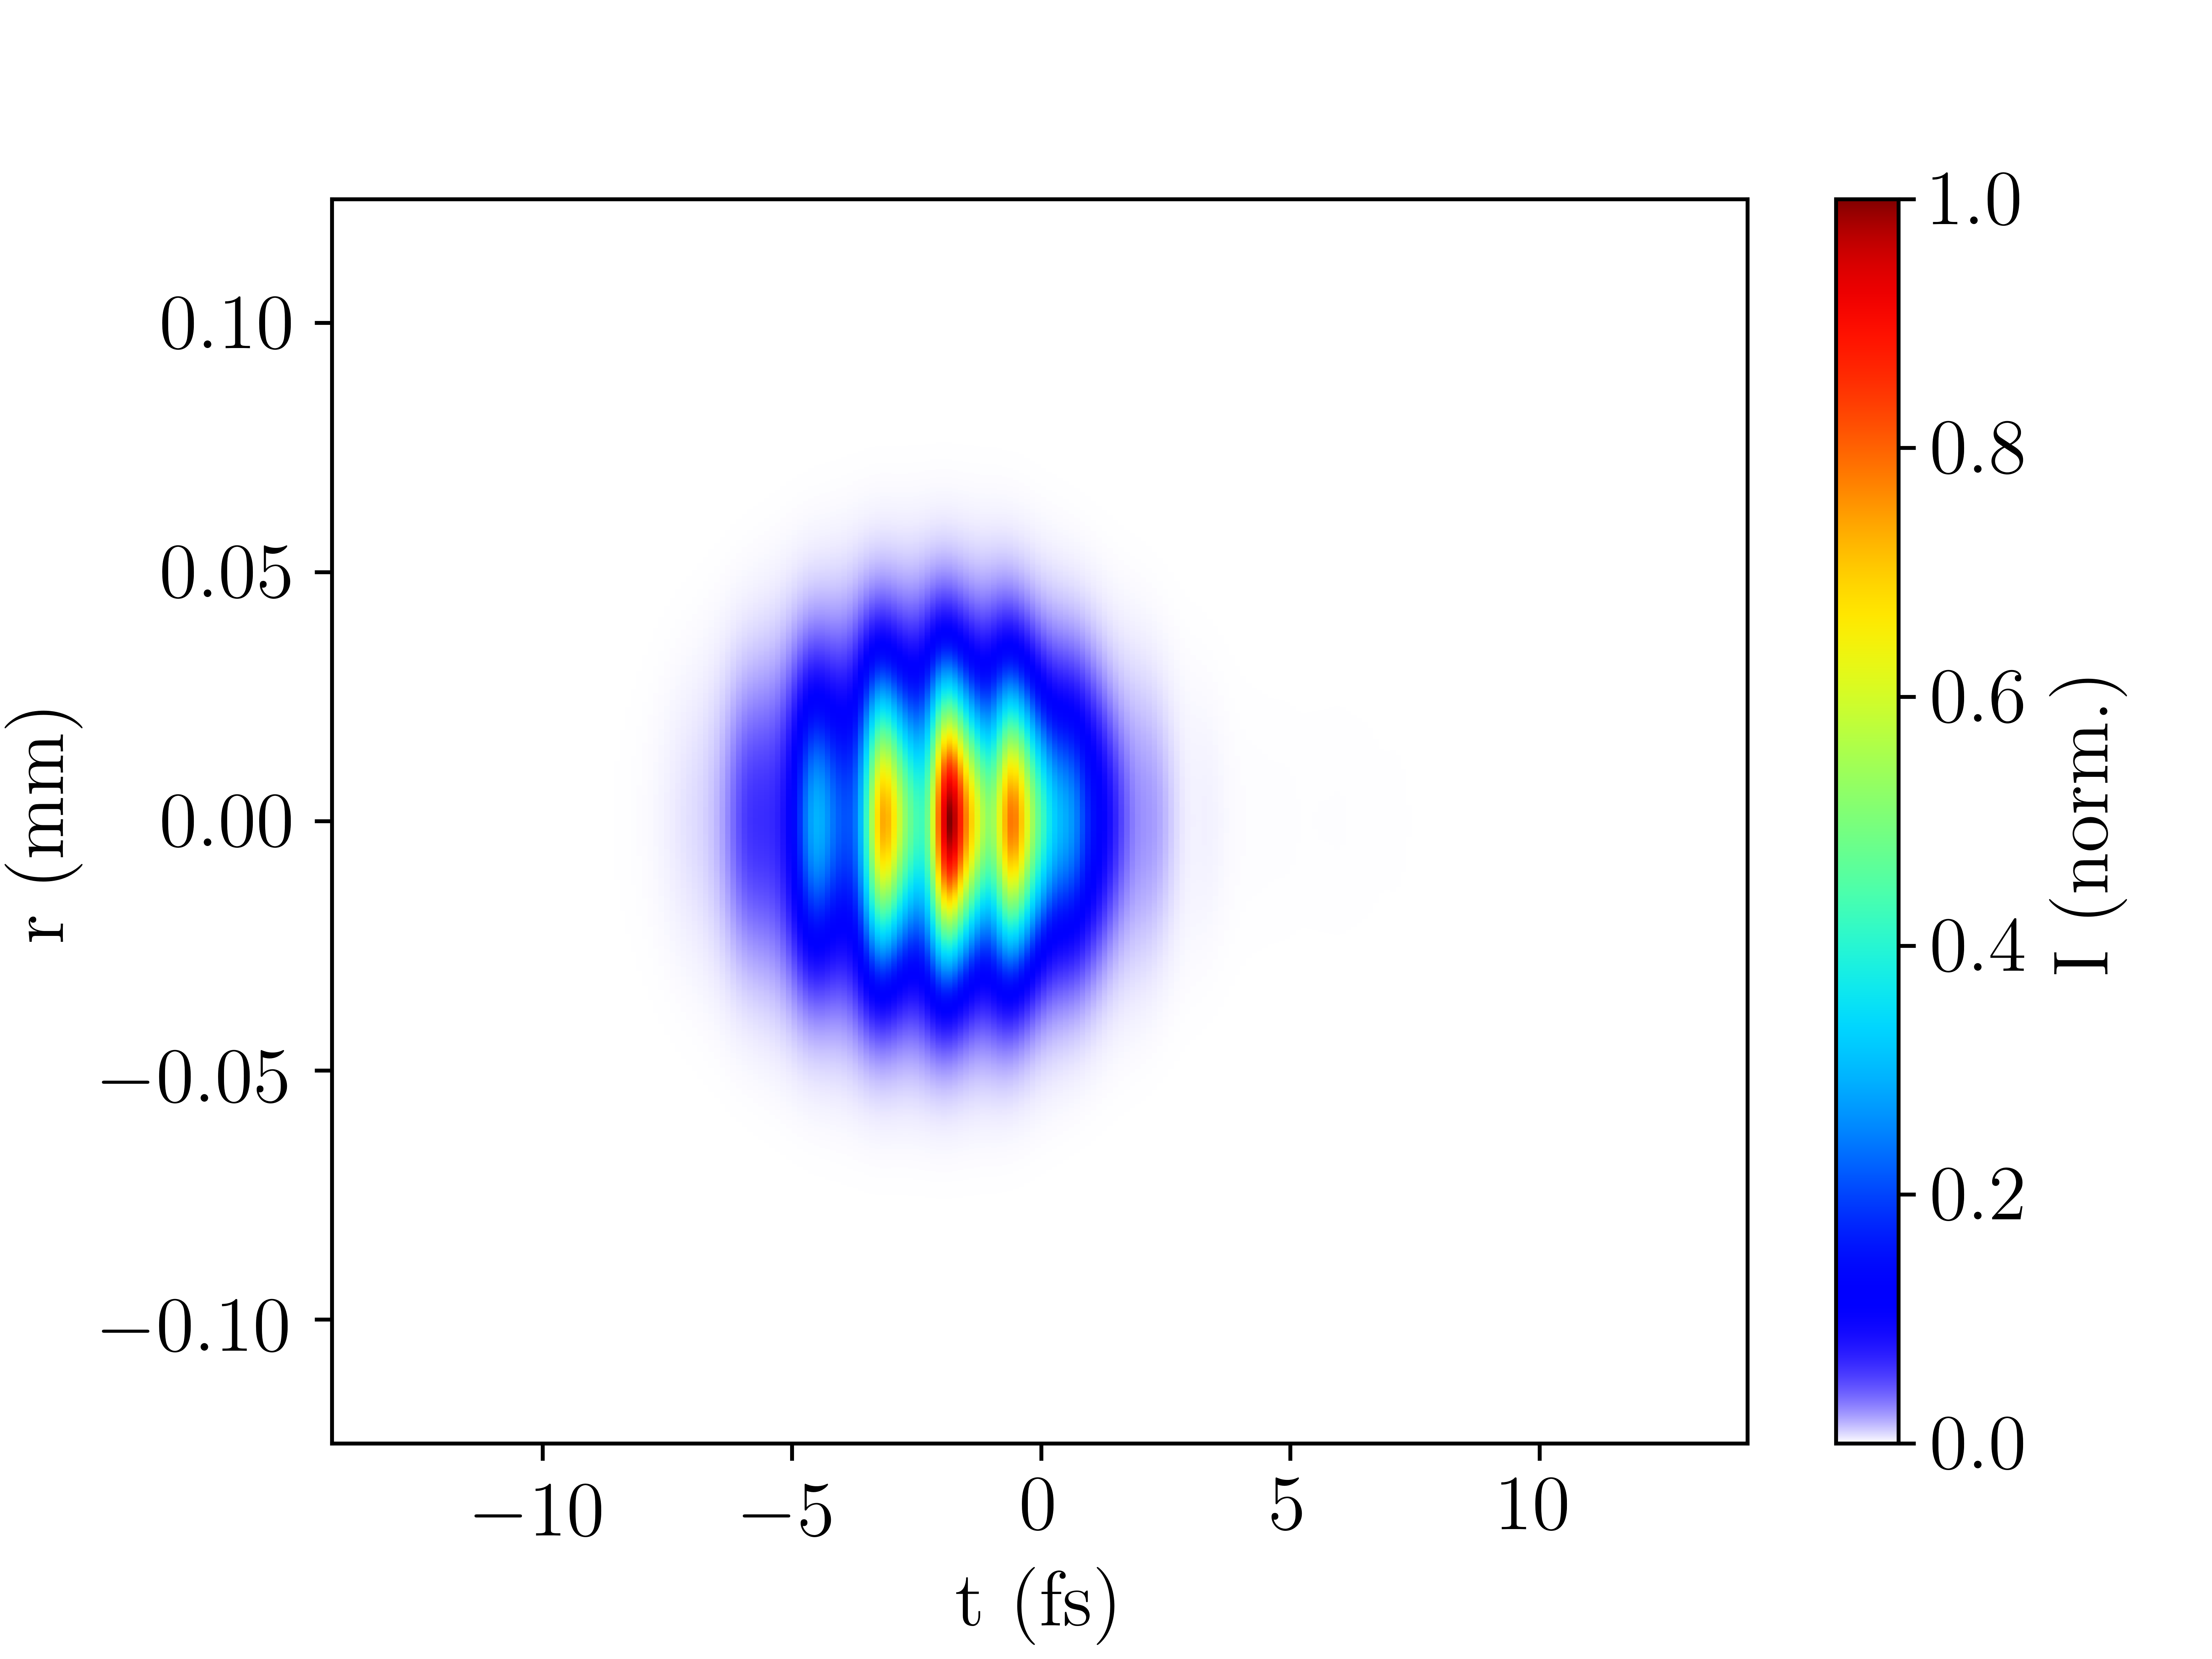
\includegraphics[width=\textwidth]{im/UV_pulse_output_Ar_no_ion}
    \caption{UV beam without ionisation}
    \end{subfigure}   
     \begin{subfigure}{0.49\textwidth}
        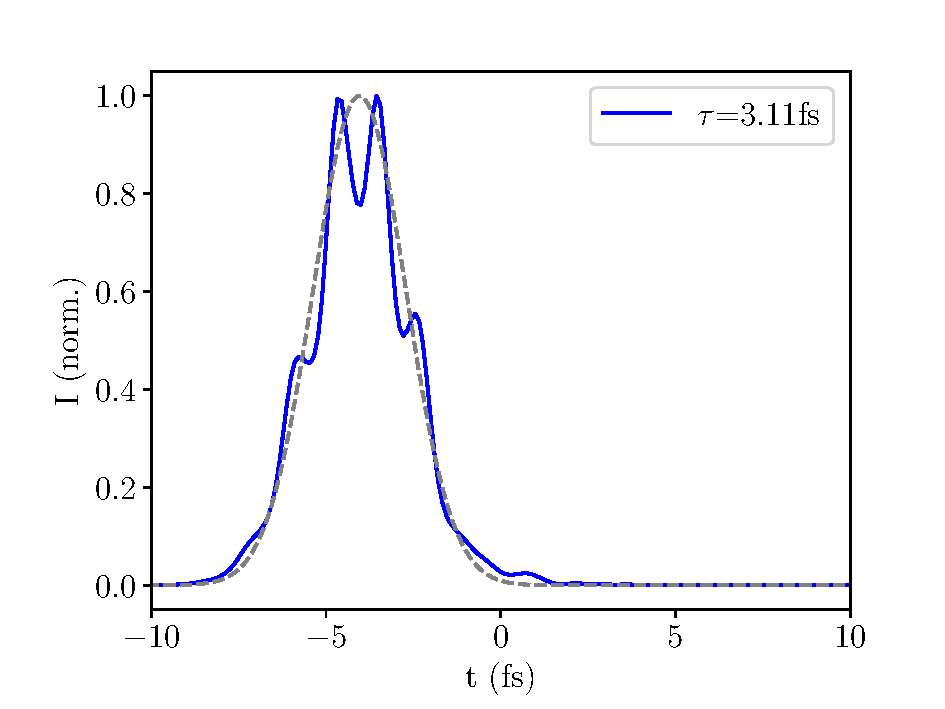
\includegraphics[width=\textwidth]{im/temporal_Ar_ion}
    \caption{UV temporal profile with ionisation}
    \end{subfigure}
    \begin{subfigure}{0.49\textwidth}
        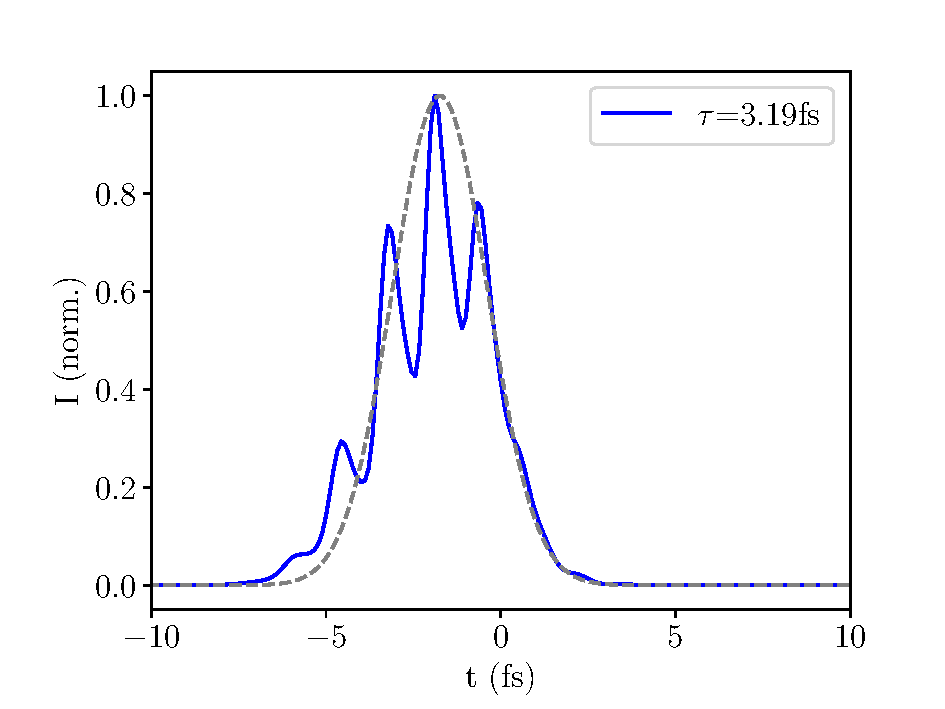
\includegraphics[width=\textwidth]{im/temporal_Ar_no_ion}
    \caption{UV temporal profile without ionisation}
    \end{subfigure}  
\caption{Simulated NIR and UV beam profiles at the output using Argon at 150mW NIR power and 0.4bar (rescaled) central pressure. Note that $\tau$ corresponds to the FWHM pulse duration.}\label{im:profile_Ar}
\end{figure*}
Figure \ref{im:prop} shows the spatiotemporal beam profile of the UV pulses at different locations throughout the gas cell. With increasing propagation distance, the originally fairly uniform pulses are deformed, resulting in the leading edge of the pulses to be more intense than the trailing edge. This is caused by trailing-edge self-defocusing of the NIR driving pulses, which confines UV generation to the leading edge of the pulse, where intensities are highest. Further investigation reveals that these effects are induced by photoionisation in the gas:  as is seen in Figure \ref{im:profile_Ar}, turning off ionisation in the simulations results in NIR as well as UV output pulses with a fairly uniform beam profile, whereas self-defocusing at the trailing edge appears when ionisation is considered. This shows that the effects of ionisation go beyond depleting UV output energies and instead actively contribute to the shaping of the output pulses. It can further be seen in Figure \ref{im:profile_Ar} that the ionisation-induced self-defocusing at the trailing edge adds to pulse compression. \par 
The findings presented above are in general agreement with similar studies carried out in the literature, such as \cite{reiter2010}.  Notably, the effects of the self-defocusing on UV pulse duration is significantly more pronounced in \cite{reiter2010} than in Figure \ref{im:profile_Ar}. This can be attributed to the different experimental conditions modelled in the two cases, specifically with respect to density distributions and input pulse characteristics like beam intensity. \par 
Due to the aforementioned limitations of the gradient density model currently used in the simulations, the results presented here regarding the effects of self-defocusing will not be an accurate description of the physical effects shaping UV generation. However, they demonstrate that the simulations, with suitable improvements, can be used to probe experimentally relevant processes that are difficult to observe directly. 

\subsection{Effects of Chirp}
Another broad application of the simulations is to explore the effects of changing different experimentally controlled parameters. Used in this way, the simulations become time-efficient tools to tune experimental conditions. Because of the lacking accuracy of the simulations at the present stage, carrying out detailed parameter scans in an attempt to find optimal conditions for UV generation would not be meaningful. Instead, this section considers a short investigation of the effects of a chirped NIR input beam as a general proof of concept of this application. For concision, only Neon is considered but equivalent results are observed for Argon. \par 
\begin{figure}[h]
\centering
 \begin{subfigure}{0.5\textwidth}
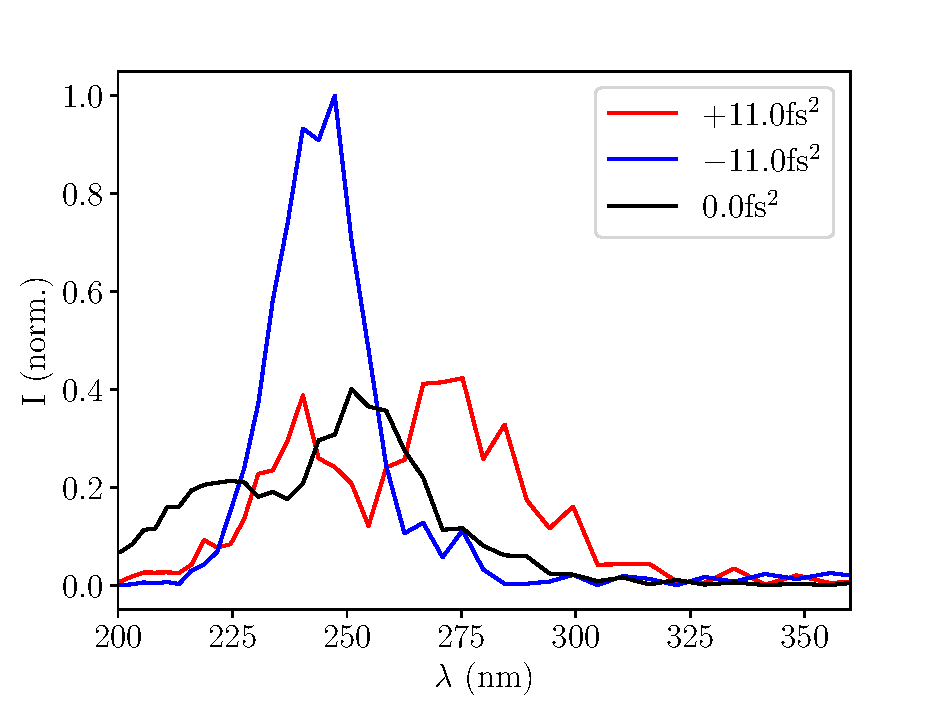
\includegraphics[width=\textwidth]{im/Ne_chirp}
\caption{}\label{im:chirp_Ar}
\end{subfigure}
 \begin{subfigure}{0.5\textwidth}
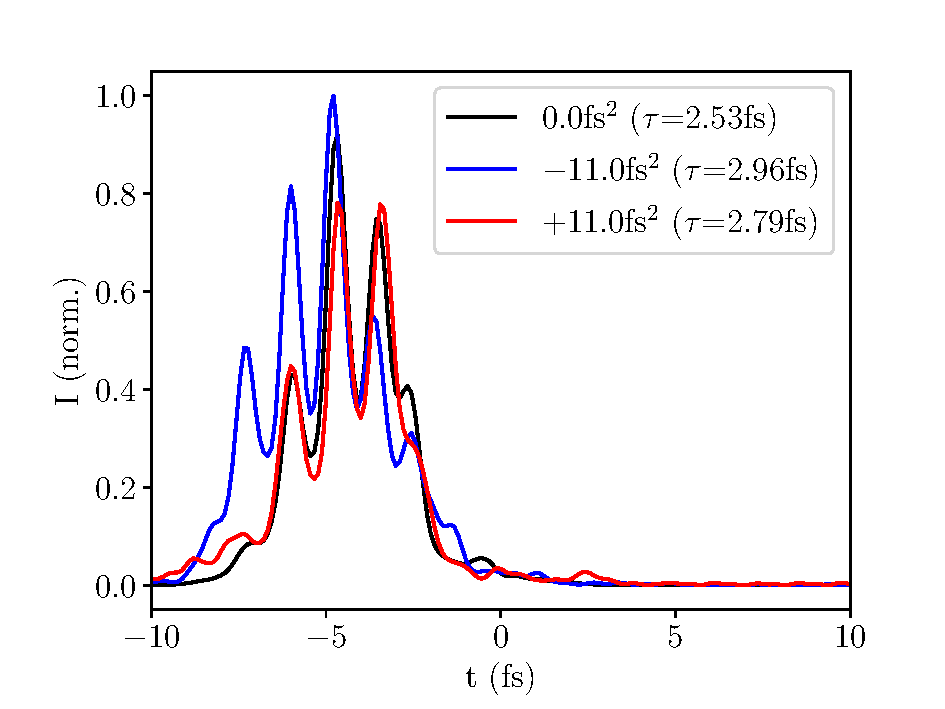
\includegraphics[width=\textwidth]{im/temporal_Ne_chirp}
\caption{}\label{im:chirp_Ne}
\end{subfigure}
\caption{Simulated UV output spectra with different GVD values for Neon at 400mW NIR power and 2.0bar (rescaled) central pressure. Note that $\tau$ corresponds to the FWHM pulse duration.}\label{im:chirp}
\end{figure}
Figure \ref{im:chirp} compares the effects on the UV output spectra of using a positively chirped, negatively chirped, or unchirped driving pulse. Evidently,  negatively chirped NIR pulses result in a more intense UV spectrum while positively chirped pulses result in spectral broadening. Considering the effects of chirp in the time domain, however, shows that the spectral broadening induced by a positively chirped NIR pulse does not translate to shorter UV pulse durations. In fact, the unchirped input pulse provides slightly shorter pulses. This indicates that the chirped input pulses also result in chirped UV pulses, increasing their time-bandwidth product and hence limiting the pulse compression that can be achieved via spectral broadening. \par 
In the next step, it would therefore be interesting to consider the spectral phase of the UV output pulses and how it is affected by a chirped input pulse. This could be used to investigate whether a suitable optical set-up can compensate the chirp on the UV pulses and hence whether the spectral broadening effects  induced by a positively chirped input pulse can be exploited for pulse compression. \par 
These findings illustrate, once again, the utility of having access to simulations of the THG process:   
investigations of the effects of varying different experimental parameters can be carried out in a time-efficient manner. This principle can, of course, be extended to a wide range of variables beyond the chirp of the input pulse. For instance, as part of this project simulations were produced to compare the UV generation properties of a variety of different gases other than Argon and Neon, including Helium, Krypton, Xenon, Oxygen, Nitrogen and N$_2$O. Additionally, the effects of driving THG with NIR pulses at different CEP values were investigated. A full analysis of these results could not be completed in the available time but it seems that Argon and Neon offer the best conditions for short but energetic UV pulses and that the CEP has only limited effects on UV spectra. 

\subsection{Comparison of Density Distributions}
As has been mentioned throughout this report, the simulation results presented so far were based on the gradient approximation of the density distribution, which only considers the central interaction region of the gas chip. This section gives an overview of the simulation results obtained when using more sophisticated gas density models. These models were produced with the \textit{COMSOL Multiphysics} software and take into account the geometry of the gas cell outside the central interaction region as well as the effects of the two pumping stages. The reason the gradient model has not yet been replaced by these \textit{COMSOL} simulations is that they currently do not sufficiently take into account the interactions of gas atoms in high-density regions due the free molecular flow models neglecting several important effects. The existing \textit{COMSOL} density models can nonetheless be used to qualitatively compare the gas distribution in the current fused silica chip to that in the previously used cell, which has a similar central interaction region but differs in the way the gas is confined and pumped. \par 
\begin{figure}[h]
\centering
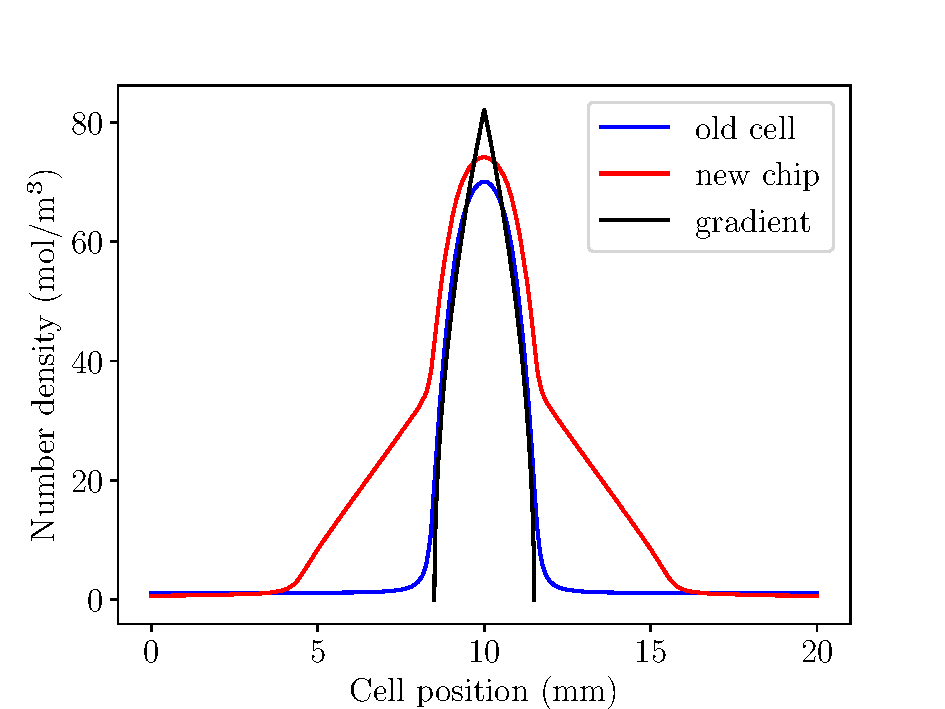
\includegraphics[width=0.5 \textwidth]{im/old_new_comp}
\caption{Comparison of the \textit{COMSOL}-generated gas density distributions of the new and old fused silica chip as well as the gradient model. The central pressure in all three cases is 2.0bar.}\label{im:dens}
\end{figure}
Figure \ref{im:dens} demonstrates that the main difference between the new chip and the old cell, at least based on the approximative \textit{COMSOL} models, is the density distribution in the roughly 5mm on either side of the central interaction region: in the new chip, the gas density drops approximately linearly while in the old cell the gas is almost entirely confined to the central interaction region. The linear density domain outside the THG region likely corresponds to the gas flowing through the laser machined channel of the new fused silica chip, as shown in Figure \ref{im:new_chip}. It is also noteworthy how closely the gradient model agrees with the density distribution of the old chip towards the edges of the central interaction region. The gradient model predicts a significantly sharper density peak than either of the two other models, however: in the new chip, and to a lesser extent also in the old chip, gas densities remain close to their peak value throughout most of the THG region. \par 
\begin{figure}[h]
\centering
 \begin{subfigure}{0.5\textwidth}
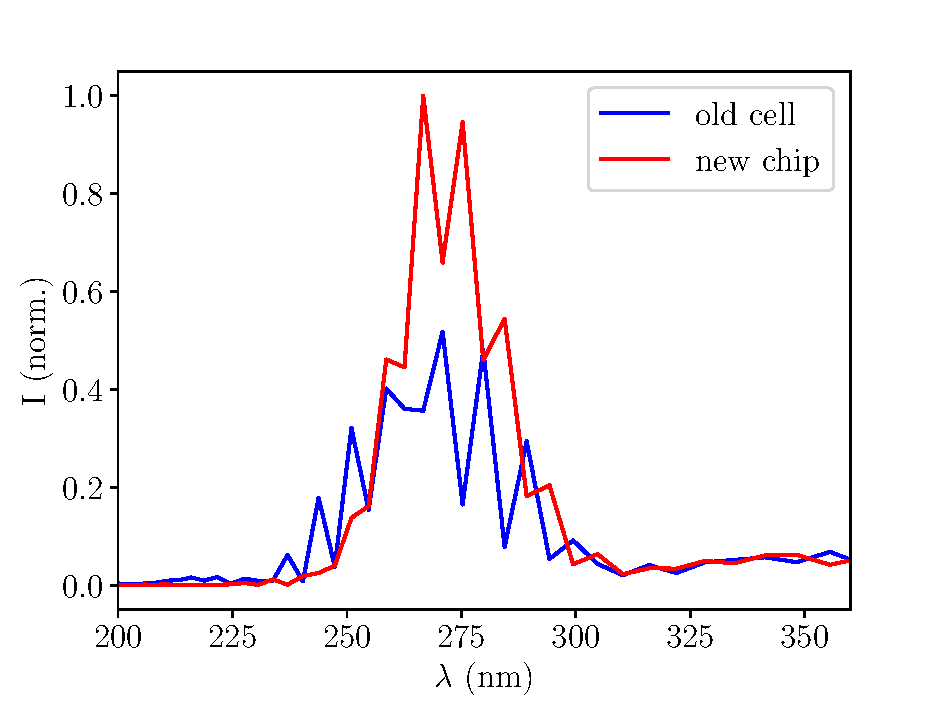
\includegraphics[width=\textwidth]{im/Ne_old_v_new}
\caption{}\label{im:coms_Ne}
\end{subfigure}
\begin{subfigure}{0.5\textwidth}
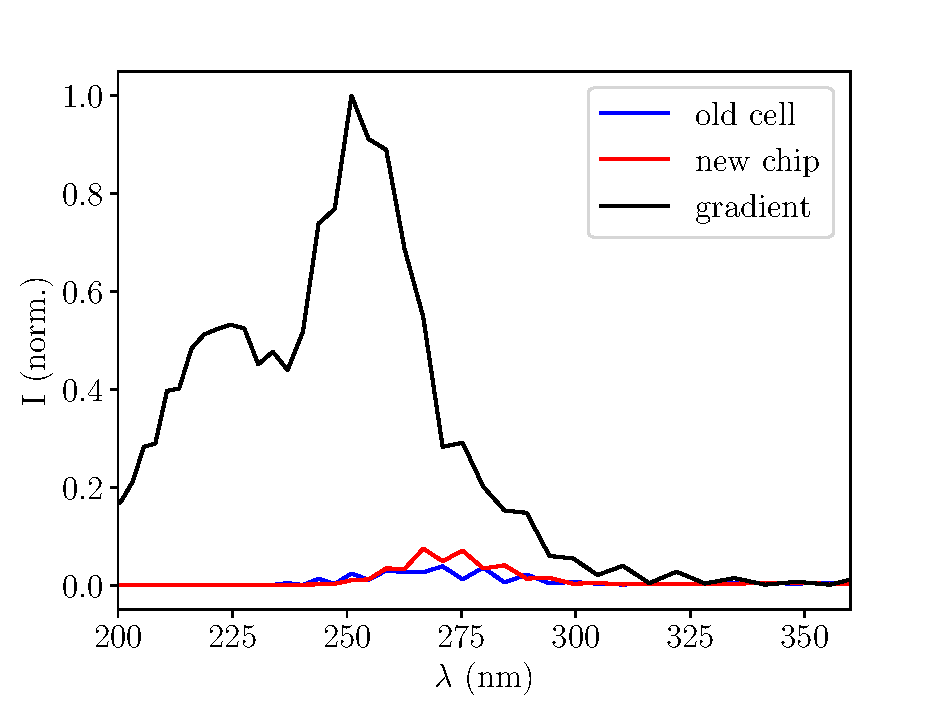
\includegraphics[width=\textwidth]{im/Ne_old_v_new_v_grad}
\caption{}\label{im:coms_Ne_grad}
\end{subfigure}
\caption{Comparison of the UV output spectra simulated for the new and old gas cells as well as the gradient model. Neon at 400mW NIR and 2.0bar (rescaled) central pressure is used.}\label{im:coms}
\end{figure}
The simulated UV spectra for propagation through the new and old cell are shown in Figure \ref{im:coms_Ne}. For concision, only results for Neon are shown, although using Argon produces equivalent output. Evidently, the new gas chip produces more intense UV pulses with a slightly broader spectrum than the old cell and is thus superior in its overall performance. These conclusions are in agreement with experimental data. Considering Figure \ref{im:dens}, the improved output using the new chip design is likely caused by the regions with linearly decreasing density on either side of the central interaction region. This implies that very tight gas confinement is not necessarily the best design strategy for UV generation in a gas cell. The effect of these linear density regions on THG and pulse shaping is one of the most interesting questions to be explored once improved \textit{COMSOL} density models can be produced. \par 
Another critical conclusion can be drawn from Figure \ref{im:coms_Ne_grad}, which superimposes the UV spectrum obtained via the gradient model on the spectra resulting from the \textit{COMSOL} gas profiles: the gradient spectrum is significantly more intense than that of both the new chip and the old cell, by a factor of roughly 10. Indeed, the simulated UV pulse energies associated  with the new chip and the old cell are of the same order of magnitude as the measured energies, whereas the gradient model predicted energies that were about 10 times too high, as mentioned previously. This is significant because Figure \ref{im:dens} clearly demonstrates that the only key difference between the gradient model and the gas distribution in the old cell is the fact that the gradient model does not take into account the regions of very low gas density outside the central interaction region. This indicates that these low-density regions significantly reduce UV output intensity, presumably via absorption or similar effects. Investigating these processes, which had previously been assumed to be negligible, is  another important task once improved simulations are available. \par 
In summary, this section demonstrated, once again, how useful the THG simulations are when it comes to understanding the UV generation process and how it is affected by various experimental parameters. While this utility is currently limited by the lack of appropriate gas density simulations, it is conceivable that the simulations could eventually be used to compare and evaluate different chip designs and aid in developing improved versions. 

\section{Outlooks}
The THG simulation package produced as part of this project yielded some promising results: qualitative agreement with experimental data and the literature could be observed. Indeed, some of the results presented in this report will be part of a manuscript submitted to the \textit{Journal of Physics: Photonics}. \par 
As was mentioned repeatedly thoughout the report, there is significant room for further improvement of the simulations. For instance, the measured spatial profile of the NIR input pulses could be fed into the simulations, replacing the Gaussian approximation as well as the assumption of radial symmetry. As the input beam shape and potential beam defects like astigmatisms have been shown experimentally to affect UV generation, it is likely that integrating this feature of the experimental conditions in the simulations would have a considerable effect. \par 
Most importantly, the THG simulations should be extended beyond the 3mm central interaction region in the chip, using a more sophisticated model for the gas density profile than the gradient approximation. As the preliminary comparison between the old and new chip in the previous section showed, the gas density profile outside the central interaction region seems to have a significant effect on UV generation.  A better model of the gas distribution, taking into account nonlinear optical effects as well as absorption outside the central chamber, would resolve the misalignment of the simulated and measured energy scales and further improve the simulation spectra. \par 
With these modifications the THG simulation code can be used to further investigate the effects presented in this report and explore a wide range of additional experimental parameters that influence UV generation and shape the output pulses.

\section{Conclusion}
This report presented simulations of the nonlinear optical processes used by the CFEL-ATTO group to produce few-femtosecond UV laser pulses. The aim of the simulations was to reproduce the relevant experimental conditions and further to give insights into the parameters and effects shaping UV generation. \par 
It has been shown that the simulations could reproduce general trends and qualitative features of measured UV spectra and energies, despite using a simplified model of the gas density distribution in the UV generation region.\par 
By considering the spatiotemporal beam profiles of both the UV and NIR pulses, it was demonstrated that ionisation-induced self-defocusing at the trailing edge contributes to pulse compression, in agreement with similar findings in the literature. \par 
Further, the simulations were shown to indicate that using chirped NIR input pulses may result in more intense UV output with broader spectra. This could be used as an additional method of pulse compression, provided the chirp on the UV output pulses can be accounted for. \par  
Additionally, using more sophisticated but still incomplete gas density models in the simulations, the performance of the fused silica chip used for gas confinement was compared to a previous design and found to be superior, in agreement with measurements. This gives important clues about the effects of the low-density regions outside the central interaction regions on the UV generation process. \par 
While the simulation software package is presently limited by the available gas density models, the results presented here are proof of its potential: with sufficient improvements, the THG simulations could become an important tool in theoretically understanding and experimentally realising the generation of few-femtosecond UV laser pulses. 

\section*{Acknowledgments}
I want to thank Josina Hahne for supervising the project and all of her support as well as Vincent Wanie for his guidance and advice. I also want to thank Chris Brahms for providing help with \textit{Luna.jl} and the entire CFEL-ATTO group for being so welcoming and friendly. Finally, thank you to Olaf Behnke and Andreas Przystawik for organising the DESY Summer Student programme. 

\section*{References}
\bibliographystyle{osa}
\bibliography{refs.bib}

\end{document}